% Created 2024-04-16 ti 18:49
% Intended LaTeX compiler: pdflatex
\documentclass[12pt]{article}

%%%% settings when exporting code %%%% 

\usepackage{listings}
\lstdefinestyle{code-small}{
backgroundcolor=\color{white}, % background color for the code block
basicstyle=\ttfamily\small, % font used to display the code
commentstyle=\color[rgb]{0.5,0,0.5}, % color used to display comments in the code
keywordstyle=\color{black}, % color used to highlight certain words in the code
numberstyle=\ttfamily\tiny\color{gray}, % color used to display the line numbers
rulecolor=\color{black}, % color of the frame
stringstyle=\color[rgb]{0,.5,0},  % color used to display strings in the code
breakatwhitespace=false, % sets if automatic breaks should only happen at whitespace
breaklines=true, % sets automatic line breaking
columns=fullflexible,
frame=single, % adds a frame around the code (non,leftline,topline,bottomline,lines,single,shadowbox)
keepspaces=true, % % keeps spaces in text, useful for keeping indentation of code
literate={~}{$\sim$}{1}, % symbol properly display via latex
numbers=none, % where to put the line-numbers; possible values are (none, left, right)
numbersep=10pt, % how far the line-numbers are from the code
showspaces=false,
showstringspaces=false,
stepnumber=1, % the step between two line-numbers. If it's 1, each line will be numbered
tabsize=1,
xleftmargin=0cm,
emph={anova,apply,class,coef,colnames,colNames,colSums,dim,dcast,for,ggplot,head,if,ifelse,is.na,lapply,list.files,library,logLik,melt,plot,require,rowSums,sapply,setcolorder,setkey,str,summary,tapply},
aboveskip = \medskipamount, % define the space above displayed listings.
belowskip = \medskipamount, % define the space above displayed listings.
lineskip = 0pt} % specifies additional space between lines in listings
\lstset{style=code-small}
%%%% packages %%%%%

\usepackage[utf8]{inputenc}
\usepackage[T1]{fontenc}
\usepackage{lmodern}
\usepackage{textcomp}
\usepackage{color}
\usepackage{graphicx}
\usepackage{grffile}
\usepackage{wrapfig}
\usepackage{rotating}
\usepackage{longtable}
\usepackage{multirow}
\usepackage{multicol}
\usepackage{changes}
\usepackage{pdflscape}
\usepackage{geometry}
\usepackage[normalem]{ulem}
\usepackage{amssymb}
\usepackage{amsmath}
\usepackage{amsfonts}
\usepackage{dsfont}
\usepackage{array}
\usepackage{ifthen}
\usepackage{hyperref}
\usepackage{natbib}
%
%%%% specifications %%%%
%
\usepackage{ifthen}
\usepackage{xifthen}
\usepackage{xargs}
\usepackage{xspace}
\newcommand\Rlogo{\textbf{\textsf{R}}\xspace} %
\RequirePackage{fancyvrb}
\DefineVerbatimEnvironment{verbatim}{Verbatim}{fontsize=\small,formatcom = {\color[rgb]{0.5,0,0}}}
\RequirePackage{colortbl} % arrayrulecolor to mix colors
\RequirePackage{setspace} % to modify the space between lines - incompatible with footnote in beamer
\renewcommand{\baselinestretch}{1.1}
\geometry{top=2cm,bottom=3cm,left=1.5cm,right=1.5cm}
\RequirePackage{changepage}
\RequirePackage{colortbl} % arrayrulecolor to mix colors
\RequirePackage{pifont}
\RequirePackage{relsize}
\newcommand{\Cross}{{\raisebox{-0.5ex}%
{\relsize{1.5}\ding{56}}}\hspace{1pt} }
\newcommand{\Valid}{{\raisebox{-0.5ex}%
{\relsize{1.5}\ding{52}}}\hspace{1pt} }
\newcommand{\CrossR}{ \textcolor{red}{\Cross} }
\newcommand{\ValidV}{ \textcolor{green}{\Valid} }
\usepackage{stackengine}
\usepackage{scalerel}
\newcommand\Warning[1][3ex]{%
\renewcommand\stacktype{L}%
\scaleto{\stackon[1.3pt]{\color{red}$\triangle$}{\tiny\bfseries !}}{#1}%
\xspace
}
\hypersetup{
citecolor=[rgb]{0,0.5,0},
urlcolor=[rgb]{0,0,0.5},
linkcolor=[rgb]{0,0,0.5},
}
\RequirePackage{epstopdf} % to be able to convert .eps to .pdf image files
\RequirePackage{capt-of} %
\RequirePackage{caption} % newlines in graphics
\RequirePackage{enumitem} % to be able to convert .eps to .pdf image files
\definecolor{light}{rgb}{1, 1, 0.9}
\definecolor{lightred}{rgb}{1.0, 0.7, 0.7}
\definecolor{lightblue}{rgb}{0.0, 0.8, 0.8}
\newcommand{\darkblue}{blue!80!black}
\newcommand{\darkgreen}{green!50!black}
\newcommand{\darkred}{red!50!black}
\usepackage{mdframed}
\newcommand{\first}{1\textsuperscript{st} }
\newcommand{\second}{2\textsuperscript{nd} }
\newcommand{\third}{3\textsuperscript{rd} }
\date{\today}
\title{Results simulation study DelayedGSD}
\hypersetup{
 colorlinks=true,
 pdfauthor={},
 pdftitle={Results simulation study DelayedGSD},
 pdfkeywords={},
 pdfsubject={},
 pdfcreator={Emacs 27.2 (Org mode 9.5.2)},
 pdflang={English}
 }
\begin{document}

\maketitle

\section{Rejection rate}
\label{sec:org9967f53}

\subsection{2 stages}
\label{sec:org441330b}
Power by method (columns) and scenario (rows): \hfill (nominal level 80\%)
\begin{verbatim}
 scenario n.sim missing binding  fixC ar method 1 method 2 method 3
        1 10000    TRUE    TRUE FALSE 10   90.43%   90.37%   90.18%
        3 10000    TRUE    TRUE FALSE  5   90.13%   90.11%   89.78%
        5 10000    TRUE    TRUE  TRUE 10   90.00%   90.10%   90.18%
        7 10000    TRUE    TRUE  TRUE  5   89.73%   89.79%   89.78%
        9  9900    TRUE   FALSE  TRUE 10   90.20%   90.33%   90.41%
       11  9900    TRUE   FALSE  TRUE  5   90.31%   90.47%   90.46%
       13  9900    TRUE   FALSE FALSE 10   90.74%   90.67%   90.41%
       15  9900    TRUE   FALSE FALSE  5   90.67%   90.66%   90.46%
       17 10000   FALSE    TRUE FALSE  5   90.38%   90.38%   90.09%
\end{verbatim}

\bigskip

Type 1 error by method (columns) and scenario (rows): \hfill (nominal level 2.5\%)
\begin{verbatim}
 scenario n.sim missing binding  fixC ar method 1 method 2 method 3
        2 10000    TRUE    TRUE FALSE 10    2.76%    2.75%    2.68%
        4 10000    TRUE    TRUE FALSE  5    2.72%    2.72%    2.70%
        6 10000    TRUE    TRUE  TRUE 10    2.56%    2.56%    2.68%
        8 10000    TRUE    TRUE  TRUE  5    2.62%    2.62%    2.70%
       10 10000    TRUE   FALSE  TRUE 10    2.14%    2.15%    2.33%
       12 10000    TRUE   FALSE  TRUE  5    2.29%    2.30%    2.34%
       14 10000    TRUE   FALSE FALSE 10    2.29%    2.27%    2.33%
       16 10000    TRUE   FALSE FALSE  5    2.36%    2.36%    2.34%
       18  9900   FALSE    TRUE FALSE  5    2.70%    2.70%    2.66%
\end{verbatim}

\clearpage

\begin{figure}[!h]
\centering
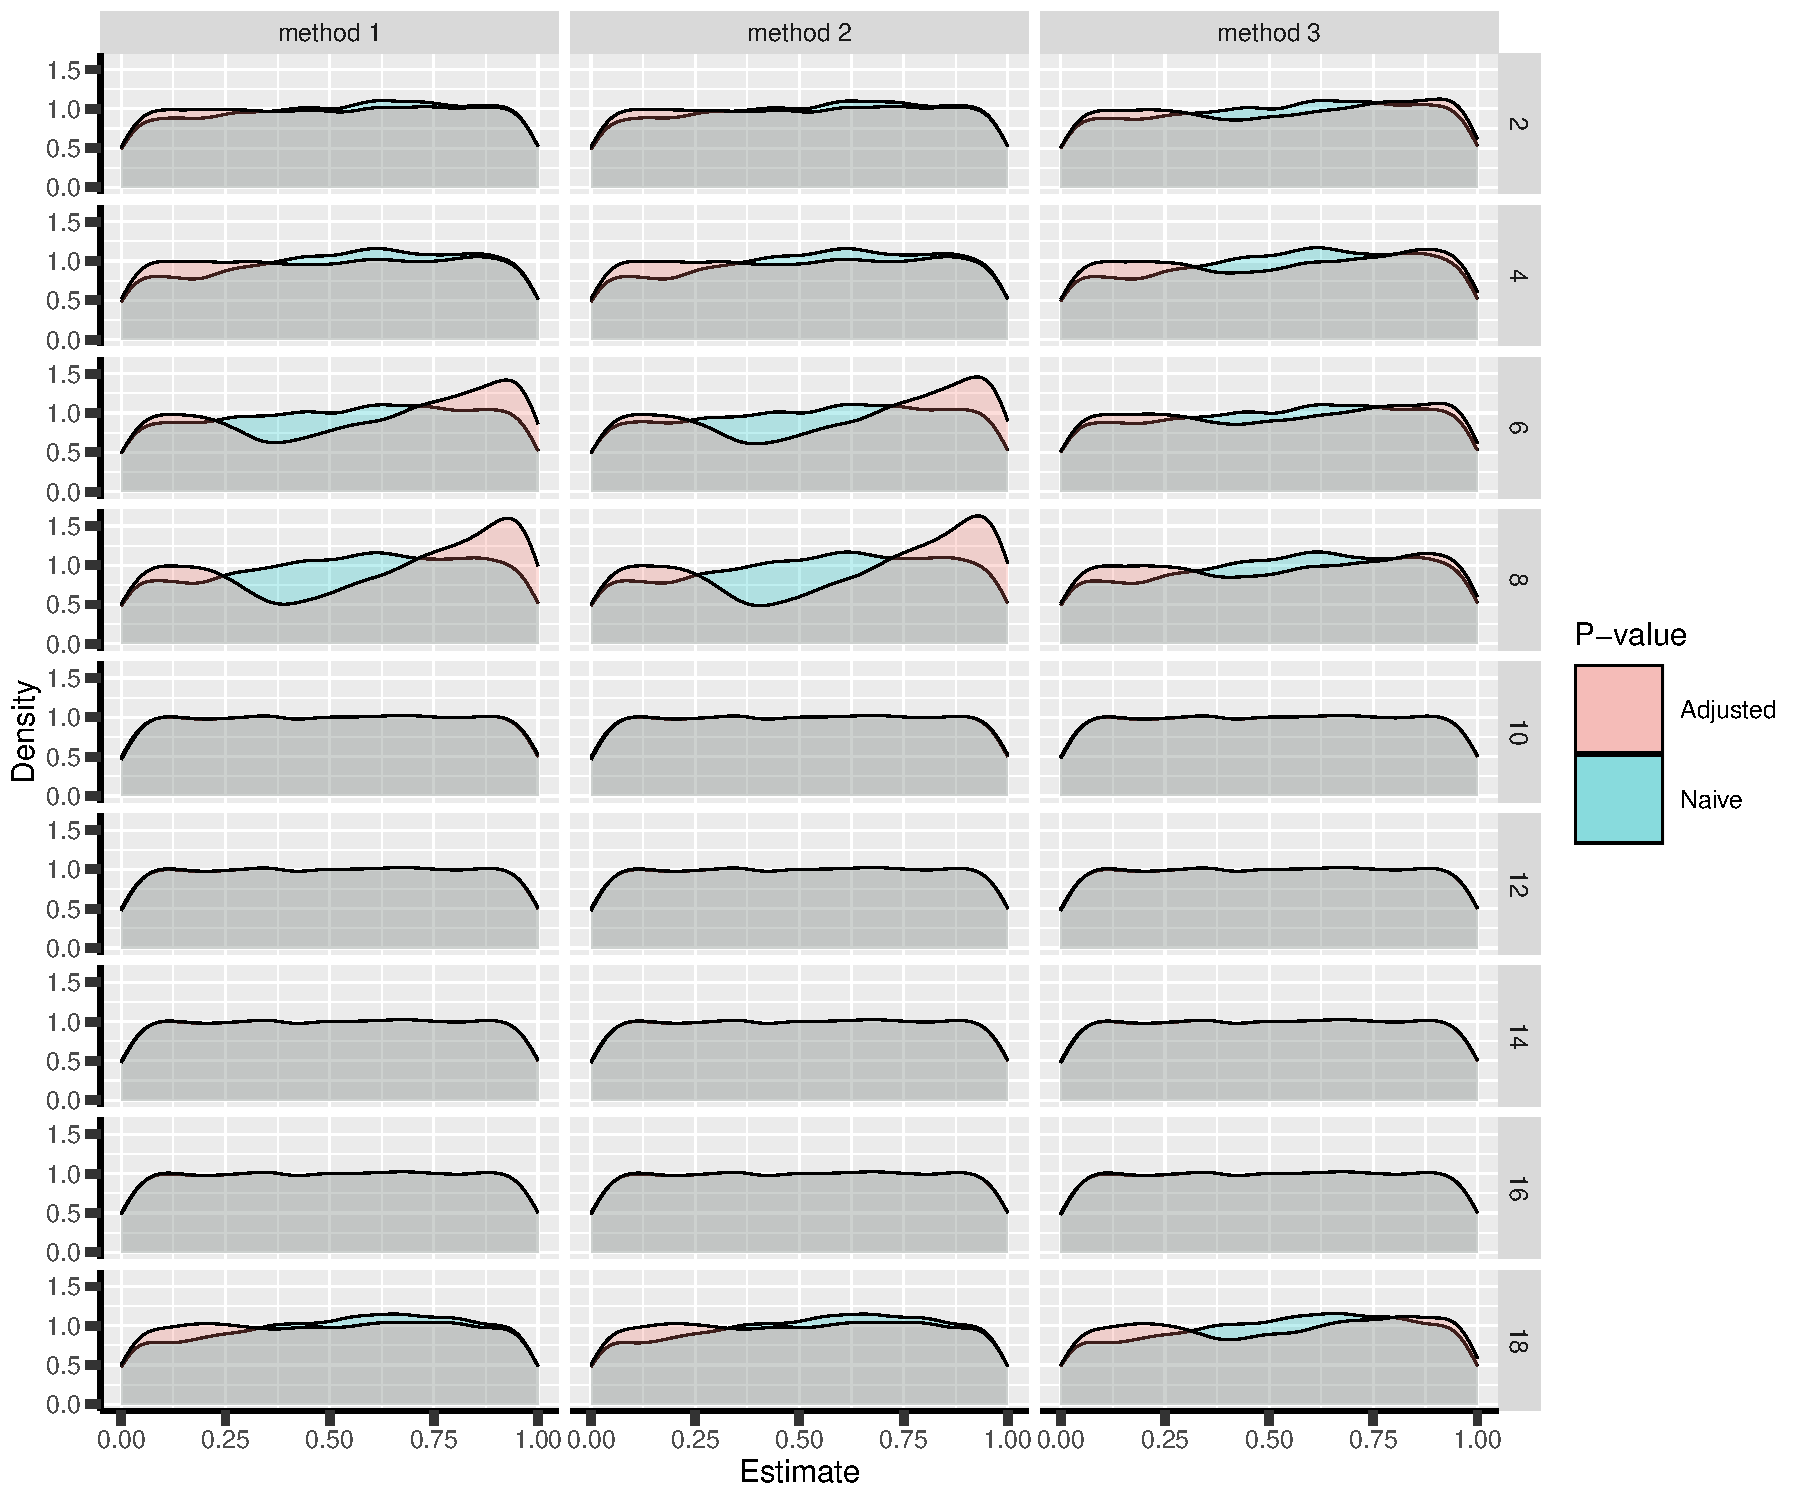
\includegraphics[trim={0 0 0 0},width=1\textwidth]{./figures/gg2stage-pvalue-density.pdf}
\caption{Naive and adjusted p-value distribution over all simulations under the null. Each row correspond to a different scenario}
\end{figure}

\begin{figure}[!h]
\centering
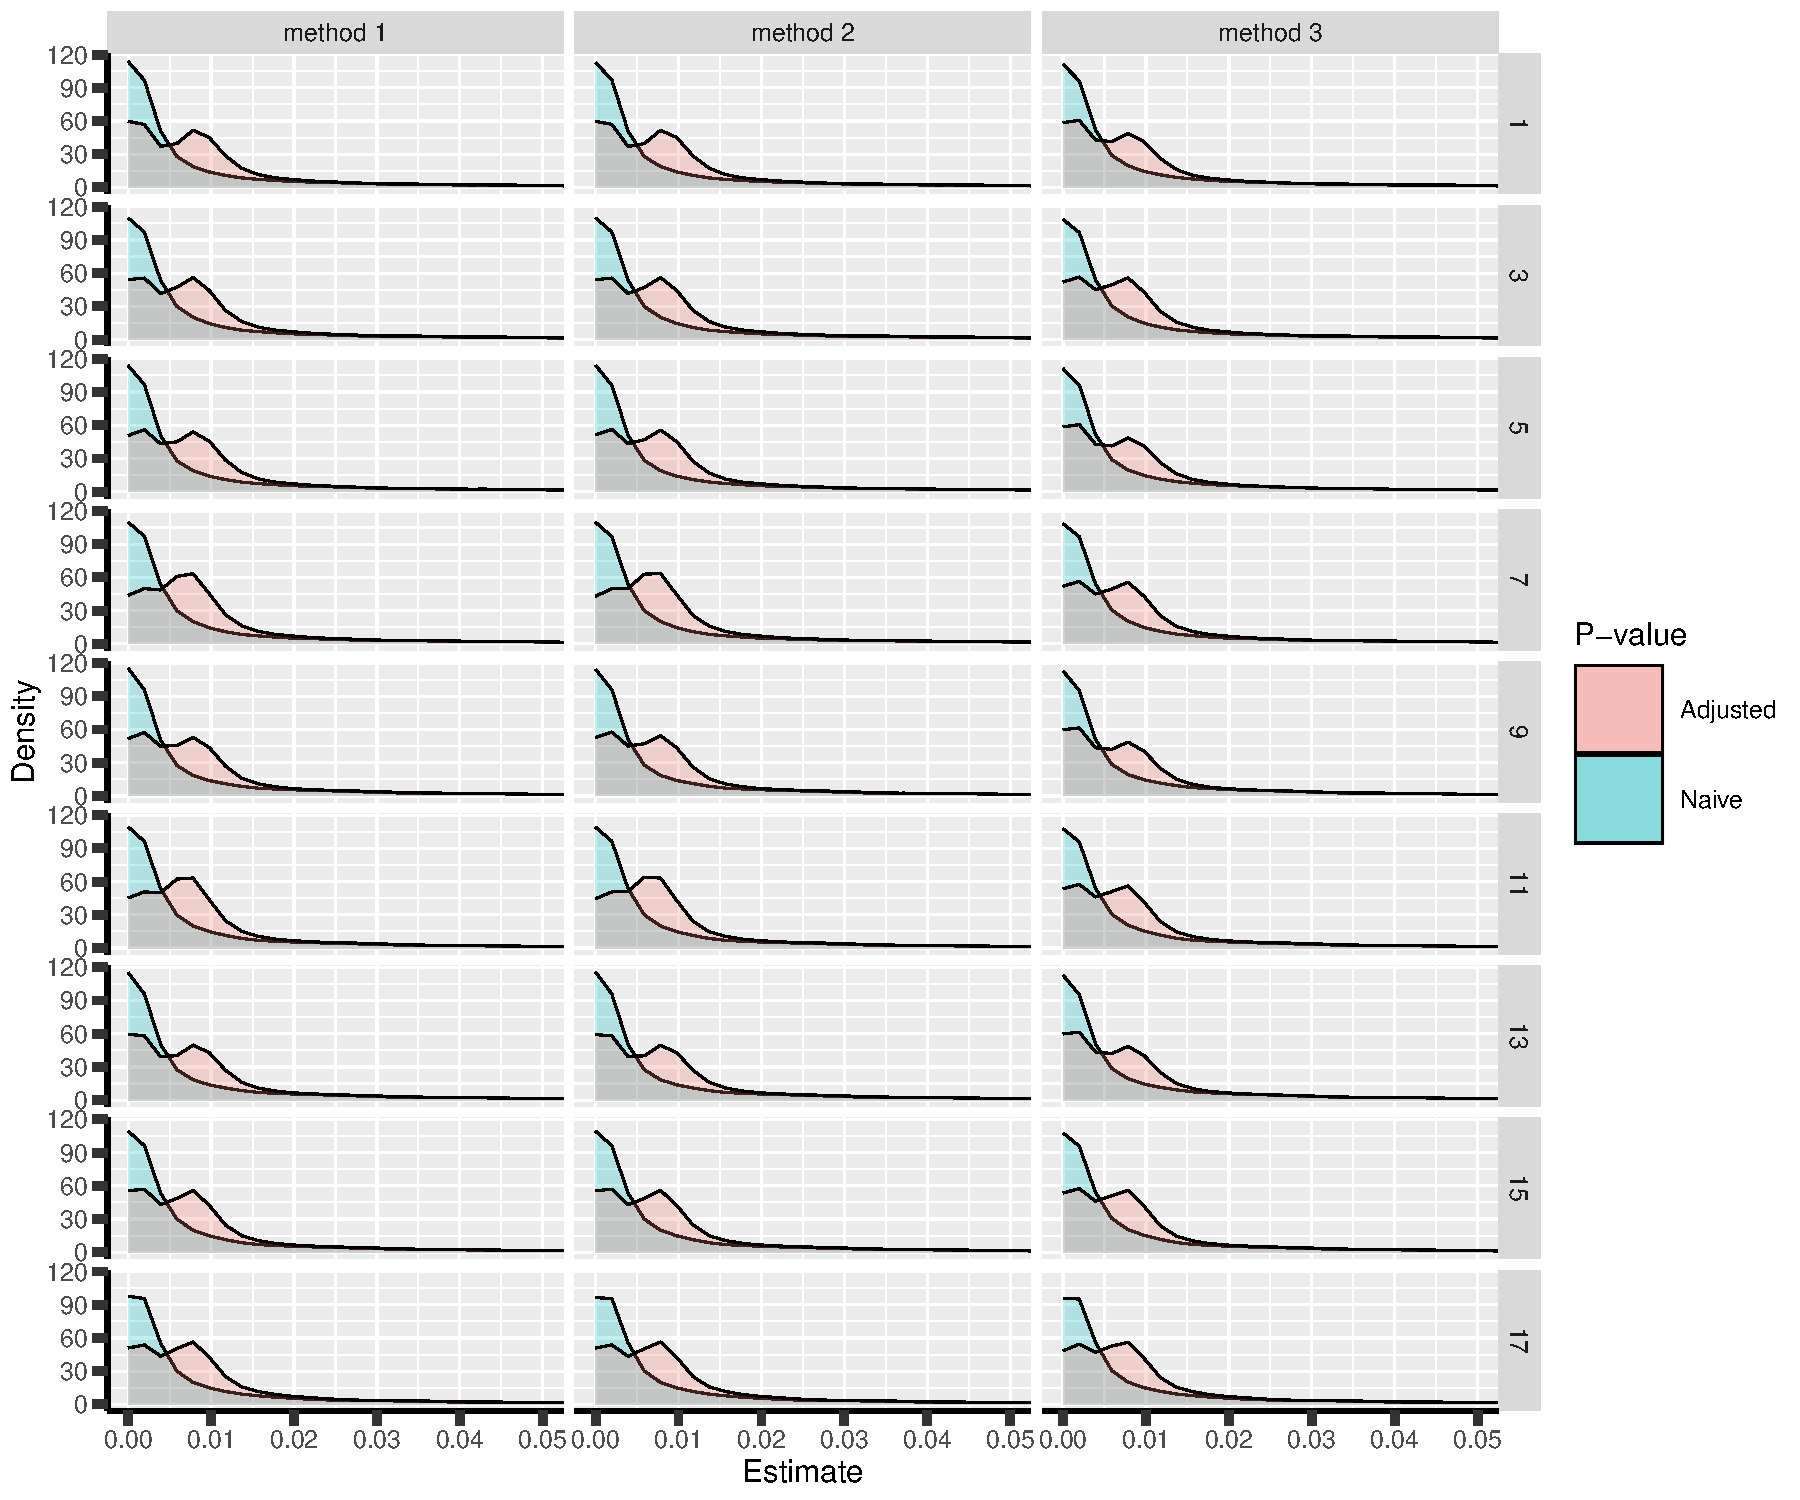
\includegraphics[trim={0 0 0 0},width=1\textwidth]{./figures/gg2stage-pvalue2-density.pdf}
\caption{Naive and adjusted p-value distribution over all simulations under the alternative. Each row correspond to a different scenario}
\end{figure}

\clearpage

\subsection{3 stages}
\label{sec:orgc266b34}

Power by method (columns) and scenario (rows): \hfill (nominal level 80\%)
\begin{verbatim}
 scenario n.sim missing binding  fixC ar method 1 method 2 method 3
        1 10000    TRUE    TRUE FALSE 10   90.96%   90.85%   90.44%
        3 10000    TRUE    TRUE FALSE  5   90.62%   90.61%   90.28%
        5 10000    TRUE    TRUE  TRUE 10   90.30%   90.44%   90.44%
        7 10000    TRUE    TRUE  TRUE  5   90.21%   90.34%   90.28%
        9 10000    TRUE   FALSE  TRUE 10   90.01%   90.27%   90.40%
       11 10000    TRUE   FALSE  TRUE  5   89.94%   90.12%   90.04%
       13 10000    TRUE   FALSE FALSE 10   90.60%   90.49%   90.40%
       15 10000    TRUE   FALSE FALSE  5   90.31%   90.31%   90.04%
       17 10000   FALSE    TRUE FALSE  5   89.85%   89.81%   89.57%
\end{verbatim}


\bigskip

Type 1 error by method (columns) and scenario (rows): \hfill (nominal level 2.5\%)
\begin{verbatim}
 scenario n.sim missing binding  fixC ar method 1 method 2 method 3
        2 10000    TRUE    TRUE FALSE 10    2.46%    2.51%    2.44%
        4 10000    TRUE    TRUE FALSE  5    2.52%    2.52%    2.49%
        6 10000    TRUE    TRUE  TRUE 10    2.25%    2.24%    2.44%
        8 10000    TRUE    TRUE  TRUE  5    2.41%    2.43%    2.49%
       10  9931    TRUE   FALSE  TRUE 10    2.30%    2.32%    2.47%
       12 10000    TRUE   FALSE  TRUE  5    2.50%    2.51%    2.64%
       14  9931    TRUE   FALSE FALSE 10    2.45%    2.42%    2.47%
       16 10000    TRUE   FALSE FALSE  5    2.52%    2.52%    2.64%
       18 10000   FALSE    TRUE FALSE  5    2.65%    2.65%    2.52%
\end{verbatim}

\clearpage

\begin{figure}[!h]
\centering
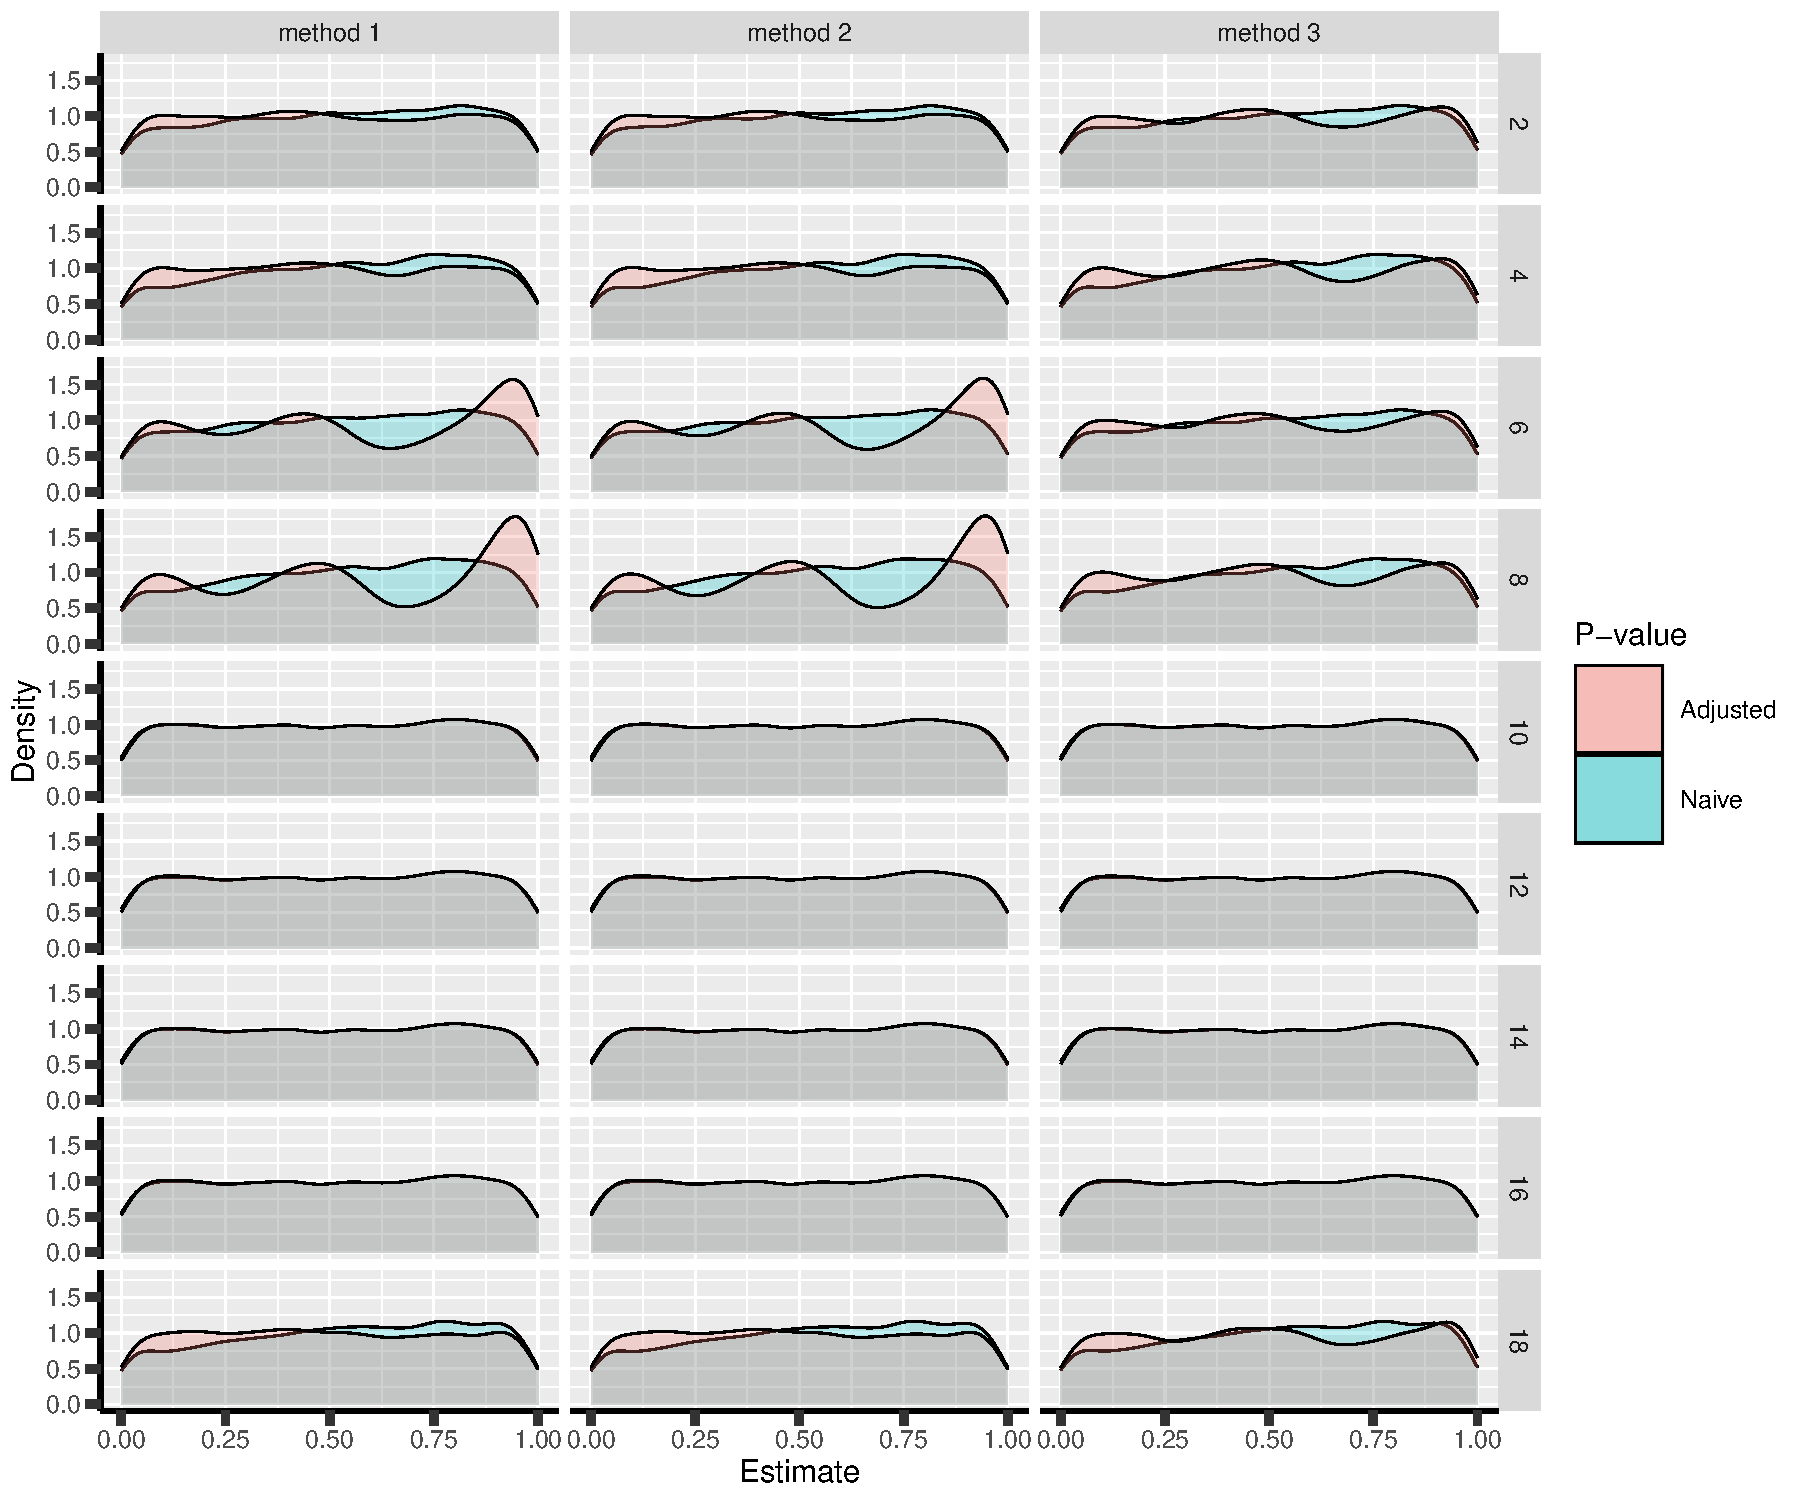
\includegraphics[trim={0 0 0 0},width=1\textwidth]{./figures/gg3stage-pvalue-density.pdf}
\caption{Naive and adjusted p-value distribution over all simulations under the null. Each row correspond to a different scenario}
\end{figure}

\begin{figure}[!h]
\centering
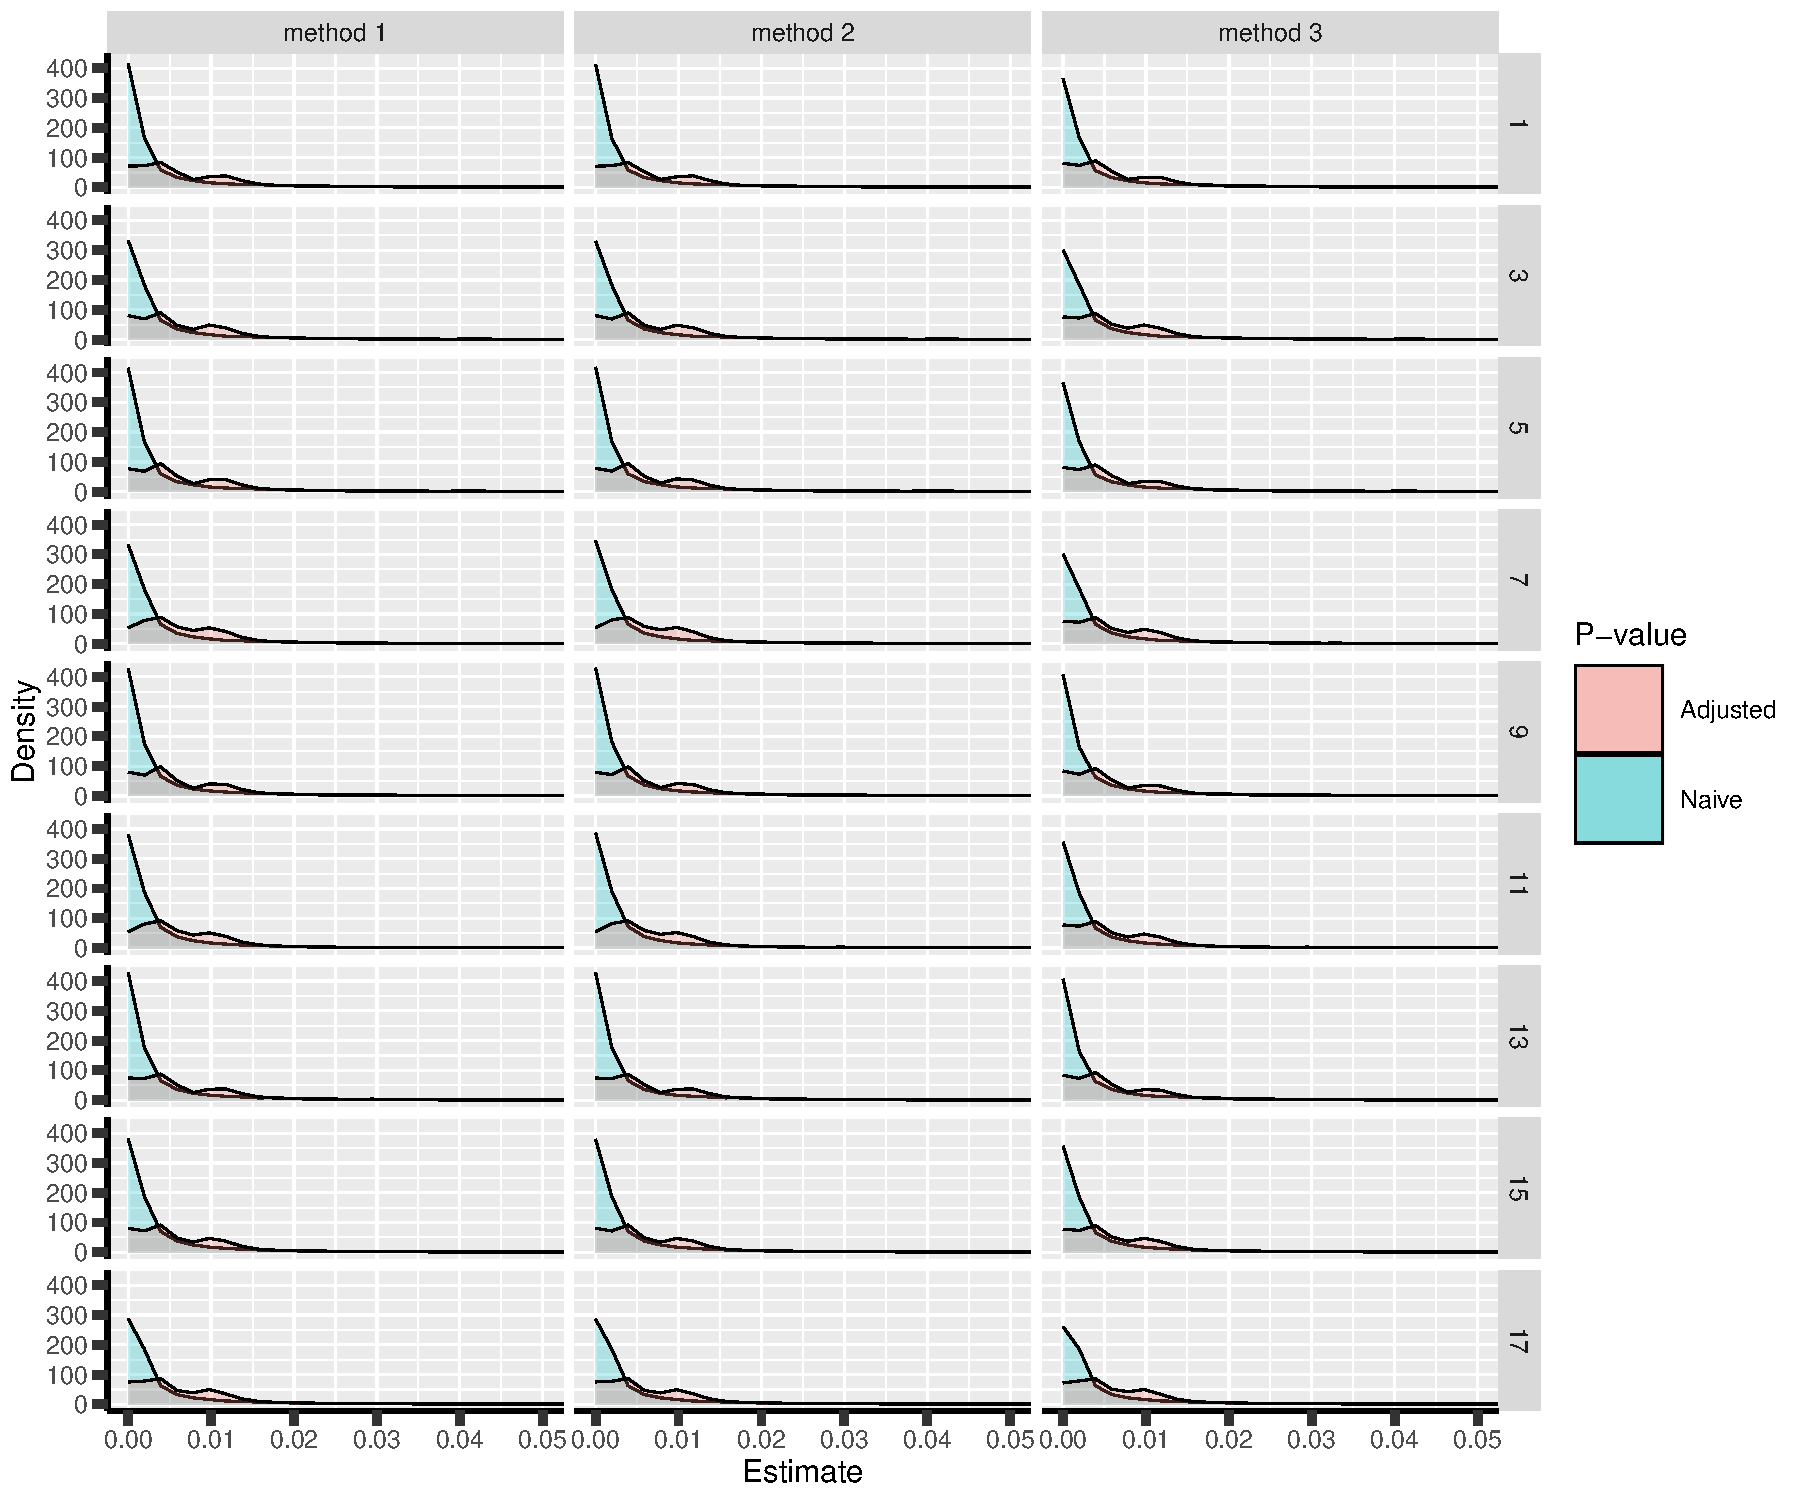
\includegraphics[trim={0 0 0 0},width=1\textwidth]{./figures/gg-pvalue2-density.pdf}
\caption{Naive and adjusted p-value distribution over all simulations under the alternative. Each row correspond to a different scenario}
\end{figure}

\clearpage

\section{Conclusion of the trial}
\label{sec:org400e8f1}

\subsection{2 stages}
\label{sec:org05c723f}
Relative frequency of stopping for efficacy/futility at decision/final

\begin{itemize}
\item Method 1
\end{itemize}
\begin{verbatim}
        N missing  hypo binding  fixC ar decision.eff decision.fut final.eff final.fut
 1: 10000    TRUE power    TRUE FALSE 10       51.23%        2.90%    39.20%     6.67%
 2: 10000    TRUE typeI    TRUE FALSE 10        0.86%       71.79%     1.90%    25.45%
 3: 10000    TRUE power    TRUE FALSE  5       48.74%        2.99%    41.39%     6.88%
 4: 10000    TRUE typeI    TRUE FALSE  5        0.81%       69.49%     1.91%    27.79%
 5: 10000    TRUE power    TRUE  TRUE 10       50.80%        3.33%    39.20%     6.67%
 6: 10000    TRUE typeI    TRUE  TRUE 10        0.66%       71.99%     1.90%    25.45%
 7: 10000    TRUE power    TRUE  TRUE  5       48.34%        3.39%    41.39%     6.88%
 8: 10000    TRUE typeI    TRUE  TRUE  5        0.71%       69.59%     1.91%    27.79%
 9:  9900    TRUE power   FALSE  TRUE 10       50.62%        3.70%    39.59%     6.10%
10: 10000    TRUE typeI   FALSE  TRUE 10        0.45%        0.23%     1.69%    97.63%
11:  9900    TRUE power   FALSE  TRUE  5       48.34%        3.47%    41.97%     6.21%
12: 10000    TRUE typeI   FALSE  TRUE  5        0.55%        0.09%     1.74%    97.62%
13:  9900    TRUE power   FALSE FALSE 10       51.15%        3.16%    39.59%     6.10%
14: 10000    TRUE typeI   FALSE FALSE 10        0.60%        0.08%     1.69%    97.63%
15:  9900    TRUE power   FALSE FALSE  5       48.70%        3.12%    41.97%     6.21%
16: 10000    TRUE typeI   FALSE FALSE  5        0.62%        0.02%     1.74%    97.62%
17: 10000   FALSE power    TRUE FALSE  5       47.04%        2.46%    43.34%     7.16%
18:  9900   FALSE typeI    TRUE FALSE  5        0.82%       67.88%     1.88%    29.42%
\end{verbatim}

\clearpage

Method 2:
\begin{verbatim}
        N missing  hypo binding  fixC ar decision.eff decision.fut final.eff final.fut
 1: 10000    TRUE power    TRUE FALSE 10       51.29%        3.13%    39.08%     6.50%
 2: 10000    TRUE typeI    TRUE FALSE 10        0.86%       72.69%     1.89%    24.56%
 3: 10000    TRUE power    TRUE FALSE  5       48.74%        3.01%    41.37%     6.88%
 4: 10000    TRUE typeI    TRUE FALSE  5        0.82%       69.59%     1.90%    27.69%
 5: 10000    TRUE power    TRUE  TRUE 10       50.50%        2.92%    39.60%     6.98%
 6: 10000    TRUE typeI    TRUE  TRUE 10        0.66%       70.13%     1.90%    27.31%
 7: 10000    TRUE power    TRUE  TRUE  5       48.22%        3.19%    41.57%     7.02%
 8: 10000    TRUE typeI    TRUE  TRUE  5        0.69%       68.11%     1.93%    29.27%
 9:  9900    TRUE power   FALSE  TRUE 10       50.46%        3.36%    39.87%     6.30%
10: 10000    TRUE typeI   FALSE  TRUE 10        0.44%        0.23%     1.71%    97.62%
11:  9900    TRUE power   FALSE  TRUE  5       48.22%        3.18%    42.25%     6.34%
12: 10000    TRUE typeI   FALSE  TRUE  5        0.55%        0.09%     1.75%    97.61%
13:  9900    TRUE power   FALSE FALSE 10       51.20%        3.32%    39.46%     6.01%
14: 10000    TRUE typeI   FALSE FALSE 10        0.58%        0.10%     1.69%    97.63%
15:  9900    TRUE power   FALSE FALSE  5       48.71%        3.14%    41.95%     6.20%
16: 10000    TRUE typeI   FALSE FALSE  5        0.62%        0.02%     1.74%    97.62%
17: 10000   FALSE power    TRUE FALSE  5       47.04%        2.46%    43.34%     7.16%
18:  9900   FALSE typeI    TRUE FALSE  5        0.82%       67.97%     1.88%    29.33%
\end{verbatim}

Method 3:
\begin{verbatim}
        N missing  hypo binding  fixC ar decision.eff decision.fut final.eff final.fut
 1: 10000    TRUE power    TRUE FALSE 10       54.76%        3.19%    35.42%     6.63%
 2: 10000    TRUE typeI    TRUE FALSE 10        0.88%       68.45%     1.80%    28.87%
 3: 10000    TRUE power    TRUE FALSE  5       49.73%        3.32%    40.05%     6.90%
 4: 10000    TRUE typeI    TRUE FALSE  5        0.80%       67.87%     1.90%    29.43%
 5: 10000    TRUE power    TRUE  TRUE 10       54.76%        3.19%    35.42%     6.63%
 6: 10000    TRUE typeI    TRUE  TRUE 10        0.88%       68.45%     1.80%    28.87%
 7: 10000    TRUE power    TRUE  TRUE  5       49.73%        3.32%    40.05%     6.90%
 8: 10000    TRUE typeI    TRUE  TRUE  5        0.80%       67.87%     1.90%    29.43%
 9:  9900    TRUE power   FALSE  TRUE 10       54.39%        3.44%    36.02%     6.14%
10: 10000    TRUE typeI   FALSE  TRUE 10        0.61%        0.36%     1.72%    97.31%
11:  9900    TRUE power   FALSE  TRUE  5       49.62%        3.29%    40.85%     6.24%
12: 10000    TRUE typeI   FALSE  TRUE  5        0.59%        0.13%     1.75%    97.53%
13:  9900    TRUE power   FALSE FALSE 10       54.39%        3.44%    36.02%     6.14%
14: 10000    TRUE typeI   FALSE FALSE 10        0.61%        0.36%     1.72%    97.31%
15:  9900    TRUE power   FALSE FALSE  5       49.62%        3.29%    40.85%     6.24%
16: 10000    TRUE typeI   FALSE FALSE  5        0.59%        0.13%     1.75%    97.53%
17: 10000   FALSE power    TRUE FALSE  5       47.93%        2.75%    42.16%     7.16%
18:  9900   FALSE typeI    TRUE FALSE  5        0.77%       66.12%     1.89%    31.22%
\end{verbatim}

\clearpage

Relative frequency of stopping for with a threshold below 1.96:
\begin{verbatim}
    scenario missing method binding  fixC ar  hypo     N rejection rejectionBelow196
 1:        1    TRUE      1    TRUE FALSE 10 power 10000    90.43%             0.43%
 2:        1    TRUE      2    TRUE FALSE 10 power 10000    90.37%             0.47%
 3:        2    TRUE      1    TRUE FALSE 10 typeI 10000     2.76%             0.20%
 4:        2    TRUE      2    TRUE FALSE 10 typeI 10000     2.75%             0.20%
 5:        3    TRUE      1    TRUE FALSE  5 power 10000    90.13%             0.40%
 6:        3    TRUE      2    TRUE FALSE  5 power 10000    90.11%             0.40%
 7:        4    TRUE      1    TRUE FALSE  5 typeI 10000     2.72%             0.10%
 8:        4    TRUE      2    TRUE FALSE  5 typeI 10000     2.72%             0.10%
 9:       13    TRUE      1   FALSE FALSE 10 power  9900    90.74%             0.54%
10:       13    TRUE      2   FALSE FALSE 10 power  9900    90.67%             0.56%
11:       14    TRUE      1   FALSE FALSE 10 typeI 10000     2.29%             0.15%
12:       14    TRUE      2   FALSE FALSE 10 typeI 10000     2.27%             0.13%
13:       15    TRUE      1   FALSE FALSE  5 power  9900    90.67%             0.35%
14:       15    TRUE      2   FALSE FALSE  5 power  9900    90.66%             0.36%
15:       16    TRUE      1   FALSE FALSE  5 typeI 10000     2.36%             0.07%
16:       16    TRUE      2   FALSE FALSE  5 typeI 10000     2.36%             0.07%
17:       17   FALSE      1    TRUE FALSE  5 power 10000    90.38%             0.43%
18:       17   FALSE      2    TRUE FALSE  5 power 10000    90.38%             0.43%
19:       18   FALSE      1    TRUE FALSE  5 typeI  9900     2.70%             0.10%
20:       18   FALSE      2    TRUE FALSE  5 typeI  9900     2.70%             0.10%
\end{verbatim}

\clearpage

\subsection{3 stages}
\label{sec:orge012e50}
Relative frequency of stopping for efficacy/futility at decision/final

\begin{itemize}
\item Method 1
\end{itemize}
\begin{verbatim}
        N missing  hypo binding  fixC ar dec1.eff dec1.fut dec2.eff dec2.fut final.eff final.fut
 1: 10000    TRUE power    TRUE FALSE 10   28.83%    1.34%   34.78%    2.69%    27.35%     5.01%
 2: 10000    TRUE typeI    TRUE FALSE 10    0.47%   47.36%    0.63%   35.07%     1.36%    15.11%
 3: 10000    TRUE power    TRUE FALSE  5   26.51%    1.38%   34.74%    2.85%    29.37%     5.15%
 4: 10000    TRUE typeI    TRUE FALSE  5    0.44%   44.88%    0.69%   35.90%     1.39%    16.70%
 5: 10000    TRUE power    TRUE  TRUE 10   28.46%    1.71%   34.49%    2.98%    27.35%     5.01%
 6: 10000    TRUE typeI    TRUE  TRUE 10    0.34%   47.49%    0.55%   35.15%     1.36%    15.11%
 7: 10000    TRUE power    TRUE  TRUE  5   26.31%    1.58%   34.53%    3.06%    29.37%     5.15%
 8: 10000    TRUE typeI    TRUE  TRUE  5    0.41%   44.91%    0.61%   35.98%     1.39%    16.70%
 9: 10000    TRUE power   FALSE  TRUE 10   28.18%    1.89%   35.13%    2.93%    26.70%     5.17%
10:  9931    TRUE typeI   FALSE  TRUE 10    0.35%    0.14%    0.49%    0.40%     1.45%    97.16%
11: 10000    TRUE power   FALSE  TRUE  5   26.02%    1.75%   35.41%    2.97%    28.51%     5.34%
12: 10000    TRUE typeI   FALSE  TRUE  5    0.42%    0.01%    0.58%    0.08%     1.50%    97.41%
13: 10000    TRUE power   FALSE FALSE 10   28.52%    1.55%   35.38%    2.68%    26.70%     5.17%
14:  9931    TRUE typeI   FALSE FALSE 10    0.44%    0.05%    0.55%    0.34%     1.45%    97.16%
15: 10000    TRUE power   FALSE FALSE  5   26.21%    1.56%   35.59%    2.79%    28.51%     5.34%
16: 10000    TRUE typeI   FALSE FALSE  5    0.43%        0    0.59%    0.07%     1.50%    97.41%
17: 10000   FALSE power    TRUE FALSE  5   25.38%    1.48%   34.27%    2.45%    30.20%     6.22%
18: 10000   FALSE typeI    TRUE FALSE  5    0.35%   42.84%    0.67%   36.11%     1.63%    18.40%
\end{verbatim}

\begin{itemize}
\item Method 2
\end{itemize}
\begin{verbatim}
        N missing  hypo binding  fixC ar dec1.eff dec1.fut dec2.eff dec2.fut final.eff final.fut
 1: 10000    TRUE power    TRUE FALSE 10   28.87%    1.42%   34.79%    2.82%    27.19%     4.91%
 2: 10000    TRUE typeI    TRUE FALSE 10    0.47%   47.79%    0.65%   35.40%     1.39%    14.30%
 3: 10000    TRUE power    TRUE FALSE  5   26.53%    1.38%   34.80%    2.86%    29.28%     5.15%
 4: 10000    TRUE typeI    TRUE FALSE  5    0.44%   44.92%    0.69%   35.99%     1.39%    16.57%
 5: 10000    TRUE power    TRUE  TRUE 10   28.18%    1.51%   34.40%    2.85%    27.86%     5.20%
 6: 10000    TRUE typeI    TRUE  TRUE 10    0.33%   44.96%    0.53%   36.43%     1.38%    16.37%
 7: 10000    TRUE power    TRUE  TRUE  5   26.18%    1.41%   34.45%    2.84%    29.71%     5.41%
 8: 10000    TRUE typeI    TRUE  TRUE  5    0.41%   43.53%    0.59%   36.40%     1.43%    17.64%
 9: 10000    TRUE power   FALSE  TRUE 10   28.03%    1.62%   35.14%    2.82%    27.10%     5.29%
10:  9931    TRUE typeI   FALSE  TRUE 10    0.35%    0.12%    0.48%    0.35%     1.48%    97.21%
11: 10000    TRUE power   FALSE  TRUE  5   25.81%    1.60%   35.45%    2.72%    28.86%     5.56%
12: 10000    TRUE typeI   FALSE  TRUE  5    0.40%    0.01%    0.59%    0.07%     1.52%    97.41%
13: 10000    TRUE power   FALSE FALSE 10   28.53%    1.61%   35.47%    2.88%    26.49%     5.02%
14:  9931    TRUE typeI   FALSE FALSE 10    0.44%    0.05%    0.52%    0.40%     1.45%    97.13%
15: 10000    TRUE power   FALSE FALSE  5   26.21%    1.56%   35.66%    2.81%    28.44%     5.32%
16: 10000    TRUE typeI   FALSE FALSE  5    0.43%        0    0.60%    0.07%     1.49%    97.41%
17: 10000   FALSE power    TRUE FALSE  5   25.42%    1.50%   34.24%    2.50%    30.15%     6.19%
18: 10000   FALSE typeI    TRUE FALSE  5    0.35%   42.87%    0.67%   36.23%     1.63%    18.25%
\end{verbatim}

\clearpage

\begin{itemize}
\item Method 3
\end{itemize}
\begin{verbatim}
        N missing  hypo binding  fixC ar dec1.eff dec1.fut dec2.eff dec2.fut final.eff final.fut
 1: 10000    TRUE power    TRUE FALSE 10   31.44%    1.68%   35.60%    2.80%    23.40%     5.08%
 2: 10000    TRUE typeI    TRUE FALSE 10    0.42%   43.69%    0.61%   36.37%     1.41%    17.50%
 3: 10000    TRUE power    TRUE FALSE  5   26.95%    1.47%   35.22%    2.96%    28.11%     5.29%
 4: 10000    TRUE typeI    TRUE FALSE  5    0.41%   43.52%    0.62%   36.31%     1.46%    17.68%
 5: 10000    TRUE power    TRUE  TRUE 10   31.44%    1.68%   35.60%    2.80%    23.40%     5.08%
 6: 10000    TRUE typeI    TRUE  TRUE 10    0.42%   43.69%    0.61%   36.37%     1.41%    17.50%
 7: 10000    TRUE power    TRUE  TRUE  5   26.95%    1.47%   35.22%    2.96%    28.11%     5.29%
 8: 10000    TRUE typeI    TRUE  TRUE  5    0.41%   43.52%    0.62%   36.31%     1.46%    17.68%
 9: 10000    TRUE power   FALSE  TRUE 10   30.84%    1.66%   36.22%    2.90%    23.34%     5.04%
10:  9931    TRUE typeI   FALSE  TRUE 10    0.41%    0.16%    0.63%    0.58%     1.42%    96.79%
11: 10000    TRUE power   FALSE  TRUE  5   26.83%    1.67%   35.85%    2.85%    27.36%     5.44%
12: 10000    TRUE typeI   FALSE  TRUE  5    0.45%    0.02%    0.67%    0.13%     1.52%    97.21%
13: 10000    TRUE power   FALSE FALSE 10   30.84%    1.66%   36.22%    2.90%    23.34%     5.04%
14:  9931    TRUE typeI   FALSE FALSE 10    0.41%    0.16%    0.63%    0.58%     1.42%    96.79%
15: 10000    TRUE power   FALSE FALSE  5   26.83%    1.67%   35.85%    2.85%    27.36%     5.44%
16: 10000    TRUE typeI   FALSE FALSE  5    0.45%    0.02%    0.67%    0.13%     1.52%    97.21%
17: 10000   FALSE power    TRUE FALSE  5   25.94%    1.64%   34.58%    2.53%    29.05%     6.26%
18: 10000   FALSE typeI    TRUE FALSE  5    0.32%   41.33%    0.62%   36.51%     1.58%    19.64%
\end{verbatim}

Relative frequency of stopping for with a threshold below 1.96:
\begin{verbatim}
    scenario missing method binding  fixC ar  hypo     N rejection rejectionBelow196
 1:        1    TRUE      1    TRUE FALSE 10 power 10000    90.96%             0.66%
 2:        1    TRUE      2    TRUE FALSE 10 power 10000    90.85%             0.62%
 3:        2    TRUE      1    TRUE FALSE 10 typeI 10000     2.46%             0.21%
 4:        2    TRUE      2    TRUE FALSE 10 typeI 10000     2.51%             0.21%
 5:        3    TRUE      1    TRUE FALSE  5 power 10000    90.62%             0.41%
 6:        3    TRUE      2    TRUE FALSE  5 power 10000    90.61%             0.42%
 7:        4    TRUE      1    TRUE FALSE  5 typeI 10000     2.52%             0.11%
 8:        4    TRUE      2    TRUE FALSE  5 typeI 10000     2.52%             0.11%
 9:       13    TRUE      1   FALSE FALSE 10 power 10000    90.60%             0.59%
10:       13    TRUE      2   FALSE FALSE 10 power 10000    90.49%             0.57%
11:       14    TRUE      1   FALSE FALSE 10 typeI  9931     2.45%             0.15%
12:       14    TRUE      2   FALSE FALSE 10 typeI  9931     2.42%             0.13%
13:       15    TRUE      1   FALSE FALSE  5 power 10000    90.31%             0.37%
14:       15    TRUE      2   FALSE FALSE  5 power 10000    90.31%             0.38%
15:       16    TRUE      1   FALSE FALSE  5 typeI 10000     2.52%             0.02%
16:       16    TRUE      2   FALSE FALSE  5 typeI 10000     2.52%             0.02%
17:       17   FALSE      1    TRUE FALSE  5 power 10000    89.85%             0.39%
18:       17   FALSE      2    TRUE FALSE  5 power 10000    89.81%             0.38%
19:       18   FALSE      1    TRUE FALSE  5 typeI 10000     2.65%             0.13%
20:       18   FALSE      2    TRUE FALSE  5 typeI 10000     2.65%             0.13%
\end{verbatim}


\clearpage

\section{Bias (True effect: 0.6 under the alternative)}
\label{sec:orgd678b31}

\subsection{2 stages}
\label{sec:org3dabc8f}
Bias per estimator and method\footnote{e.g. \texttt{biasMLE1} mixed model
estimator (treatment effect), method 1 (boundaries)}:
\begin{adjustwidth}{-1cm}{-1cm}
\begin{verbatim}
     hypo missing binding  fixC ar biasMLE1 biasMLE2 biasMLE3 biasMUE1 biasMUE2 biasMUE3
 1: power    TRUE    TRUE FALSE 10  0.01251  0.01233  0.01275  0.00470  0.00452 -0.00450
 2: typeI    TRUE    TRUE FALSE 10 -0.01673 -0.01655 -0.01713 -0.00518 -0.00508 -0.01539
 3: power    TRUE    TRUE FALSE  5  0.02412  0.02410  0.02442  0.01141  0.01138  0.00302
 4: typeI    TRUE    TRUE FALSE  5 -0.02839 -0.02837 -0.02897 -0.01206 -0.01207 -0.02288
 5: power    TRUE    TRUE  TRUE 10  0.01251  0.01278  0.01275 -0.01829 -0.01939 -0.00450
 6: typeI    TRUE    TRUE  TRUE 10 -0.01673 -0.01725 -0.01713 -0.04244 -0.04509 -0.01539
 7: power    TRUE    TRUE  TRUE  5  0.02412  0.02444  0.02442 -0.02060 -0.02149  0.00302
 8: typeI    TRUE    TRUE  TRUE  5 -0.02839 -0.02907 -0.02897 -0.06515 -0.06704 -0.02288
 9: power    TRUE   FALSE  TRUE 10  0.01191  0.01234  0.01241 -0.00291 -0.00536  0.01012
10: typeI    TRUE   FALSE  TRUE 10 -0.00049 -0.00049 -0.00029 -0.00156 -0.00154  0.00000
11: power    TRUE   FALSE  TRUE  5  0.02382  0.02410  0.02409 -0.00384 -0.00573  0.01884
12: typeI    TRUE   FALSE  TRUE  5 -0.00004 -0.00004  0.00004 -0.00057 -0.00056 -0.00010
13: power    TRUE   FALSE FALSE 10  0.01191  0.01174  0.01241  0.01785  0.01836  0.01012
14: typeI    TRUE   FALSE FALSE 10 -0.00049 -0.00049 -0.00029 -0.00060 -0.00072  0.00000
15: power    TRUE   FALSE FALSE  5  0.02382  0.02379  0.02409  0.02577  0.02582  0.01884
16: typeI    TRUE   FALSE FALSE  5 -0.00004 -0.00004  0.00004 -0.00002 -0.00002 -0.00010
17: power   FALSE    TRUE FALSE  5  0.02542  0.02542  0.02598  0.01365  0.01366  0.00371
18: typeI   FALSE    TRUE FALSE  5 -0.02471 -0.02472 -0.02520 -0.00941 -0.00941 -0.02205
\end{verbatim}
\end{adjustwidth}

Median bias \footnote{Relative frequency at which the estimate is greater than the truth minus 0.5} per estimator and method:
\begin{adjustwidth}{-1cm}{-1cm}
\begin{verbatim}
     hypo missing binding  fixC ar mbiasMLE1 mbiasMLE2 mbiasMLE3 mbiasMUE1 mbiasMUE2 mbiasMUE3
 1: power    TRUE    TRUE FALSE 10    0.0218    0.0218    0.0198  -0.00560  -0.00550  -0.01340
 2: typeI    TRUE    TRUE FALSE 10   -0.0272   -0.0265   -0.0296  -0.00520  -0.00606  -0.02692
 3: power    TRUE    TRUE FALSE  5    0.0472    0.0472    0.0471  -0.00425  -0.00425  -0.00760
 4: typeI    TRUE    TRUE FALSE  5   -0.0446   -0.0444   -0.0478  -0.00700  -0.00746  -0.02836
 5: power    TRUE    TRUE  TRUE 10    0.0218    0.0216    0.0198  -0.02751  -0.02951  -0.01340
 6: typeI    TRUE    TRUE  TRUE 10   -0.0272   -0.0292   -0.0296  -0.08467  -0.08715  -0.02692
 7: power    TRUE    TRUE  TRUE  5    0.0472    0.0471    0.0471  -0.02956  -0.03136  -0.00760
 8: typeI    TRUE    TRUE  TRUE  5   -0.0446   -0.0472   -0.0478  -0.10726  -0.10396  -0.02836
 9: power    TRUE   FALSE  TRUE 10    0.0256    0.0257    0.0261  -0.00808  -0.01103   0.00434
10: typeI    TRUE   FALSE  TRUE 10   -0.0040   -0.0040   -0.0040  -0.00516  -0.00516  -0.00301
11: power    TRUE   FALSE  TRUE  5    0.0499    0.0495    0.0503  -0.01402  -0.01674   0.00559
12: typeI    TRUE   FALSE  TRUE  5   -0.0040   -0.0040   -0.0040  -0.00455  -0.00455  -0.00396
13: power    TRUE   FALSE FALSE 10    0.0256    0.0256    0.0261   0.01372   0.01458   0.00434
14: typeI    TRUE   FALSE FALSE 10   -0.0040   -0.0040   -0.0040  -0.00440  -0.00450  -0.00301
15: power    TRUE   FALSE FALSE  5    0.0499    0.0499    0.0503   0.00871   0.00881   0.00559
16: typeI    TRUE   FALSE FALSE  5   -0.0040   -0.0040   -0.0040  -0.00420  -0.00420  -0.00396
17: power   FALSE    TRUE FALSE  5    0.0479    0.0479    0.0481  -0.00425  -0.00435  -0.01240
18: typeI   FALSE    TRUE FALSE  5   -0.0417   -0.0418   -0.0437  -0.00425  -0.00445  -0.02922
\end{verbatim}

\end{adjustwidth}

\clearpage

\subsection{3 stages}
\label{sec:orgeec01bf}
Bias per estimator and method\footnote{e.g. \texttt{biasMLE1} mixed model
estimator (treatment effect), method 1 (boundaries)}:
\begin{adjustwidth}{-1cm}{-1cm}
\begin{verbatim}
     hypo missing binding  fixC ar biasMLE1 biasMLE2 biasMLE3 biasMUE1 biasMUE2 biasMUE3
 1: power    TRUE    TRUE FALSE 10   0.0240   0.0238   0.0255   0.0161   0.0159   0.0074
 2: typeI    TRUE    TRUE FALSE 10  -0.0281  -0.0279  -0.0280  -0.0134  -0.0129  -0.0249
 3: power    TRUE    TRUE FALSE  5   0.0380   0.0380   0.0388   0.0216   0.0217   0.0130
 4: typeI    TRUE    TRUE FALSE  5  -0.0447  -0.0447  -0.0448  -0.0226  -0.0226  -0.0348
 5: power    TRUE    TRUE  TRUE 10   0.0240   0.0245   0.0255  -0.0076  -0.0083   0.0074
 6: typeI    TRUE    TRUE  TRUE 10  -0.0281  -0.0283  -0.0280  -0.0562  -0.0582  -0.0249
 7: power    TRUE    TRUE  TRUE  5   0.0380   0.0386   0.0388  -0.0105  -0.0104   0.0130
 8: typeI    TRUE    TRUE  TRUE  5  -0.0447  -0.0449  -0.0448  -0.0848  -0.0859  -0.0348
 9: power    TRUE   FALSE  TRUE 10   0.0242   0.0246   0.0253   0.0150   0.0129   0.0274
10: typeI    TRUE   FALSE  TRUE 10   0.0024   0.0023   0.0027   0.0010   0.0011   0.0031
11: power    TRUE   FALSE  TRUE  5   0.0380   0.0385   0.0388   0.0133   0.0112   0.0353
12: typeI    TRUE   FALSE  TRUE  5   0.0035   0.0035   0.0038   0.0029   0.0029   0.0038
13: power    TRUE   FALSE FALSE 10   0.0242   0.0241   0.0253   0.0348   0.0356   0.0274
14: typeI    TRUE   FALSE FALSE 10   0.0024   0.0024   0.0027   0.0021   0.0019   0.0031
15: power    TRUE   FALSE FALSE  5   0.0380   0.0380   0.0388   0.0427   0.0428   0.0353
16: typeI    TRUE   FALSE FALSE  5   0.0035   0.0035   0.0038   0.0032   0.0033   0.0038
17: power   FALSE    TRUE FALSE  5   0.0373   0.0372   0.0379   0.0221   0.0220   0.0122
18: typeI   FALSE    TRUE FALSE  5  -0.0420  -0.0419  -0.0423  -0.0203  -0.0202  -0.0344
\end{verbatim}
\end{adjustwidth}

Median bias \footnote{Relative frequency at which the estimate is greater than the truth minus 0.5} per estimator and method:
\begin{adjustwidth}{-1cm}{-1cm}
\begin{verbatim}
     hypo missing binding  fixC ar mbiasMLE1 mbiasMLE2 mbiasMLE3 mbiasMUE1 mbiasMUE2 mbiasMUE3
 1: power    TRUE    TRUE FALSE 10    0.0348    0.0346    0.0360   0.00130   0.00120   -0.0128
 2: typeI    TRUE    TRUE FALSE 10   -0.0428   -0.0423   -0.0426   0.00205   0.00200   -0.0161
 3: power    TRUE    TRUE FALSE  5    0.0577    0.0576    0.0573  -0.00085  -0.00085   -0.0185
 4: typeI    TRUE    TRUE FALSE  5   -0.0589   -0.0588   -0.0589  -0.00455  -0.00415   -0.0195
 5: power    TRUE    TRUE  TRUE 10    0.0348    0.0350    0.0360  -0.03457  -0.03658   -0.0128
 6: typeI    TRUE    TRUE  TRUE 10   -0.0428   -0.0426   -0.0426  -0.02798  -0.03293   -0.0161
 7: power    TRUE    TRUE  TRUE  5    0.0577    0.0578    0.0573  -0.05581  -0.05901   -0.0185
 8: typeI    TRUE    TRUE  TRUE  5   -0.0589   -0.0589   -0.0589  -0.04987  -0.05342   -0.0192
 9: power    TRUE   FALSE  TRUE 10    0.0413    0.0408    0.0420  -0.00557  -0.01015    0.0046
10: typeI    TRUE   FALSE  TRUE 10    0.0012    0.0012    0.0012  -0.00101  -0.00066    0.0026
11: power    TRUE   FALSE  TRUE  5    0.0633    0.0633    0.0629  -0.03128  -0.03685    0.0062
12: typeI    TRUE   FALSE  TRUE  5    0.0015    0.0015    0.0015   0.00075   0.00070    0.0023
13: power    TRUE   FALSE FALSE 10    0.0413    0.0415    0.0420   0.02261   0.02398    0.0046
14: typeI    TRUE   FALSE FALSE 10    0.0012    0.0012    0.0012  -0.00025  -0.00010    0.0026
15: power    TRUE   FALSE FALSE  5    0.0633    0.0630    0.0629   0.02410   0.02421    0.0063
16: typeI    TRUE   FALSE FALSE  5    0.0015    0.0015    0.0015   0.00085   0.00075    0.0022
17: power   FALSE    TRUE FALSE  5    0.0584    0.0586    0.0585   0.00285   0.00275   -0.0157
18: typeI   FALSE    TRUE FALSE  5   -0.0589   -0.0584   -0.0587   0.00190   0.00230   -0.0117
\end{verbatim}

\end{adjustwidth}

\clearpage

\section{Distribution of the estimates}
\label{sec:orgb9b4e7e}

\subsection{2 stages}
\label{sec:org53f93db}
Distribution of the estimates:
\begin{figure}[!h]
\centering
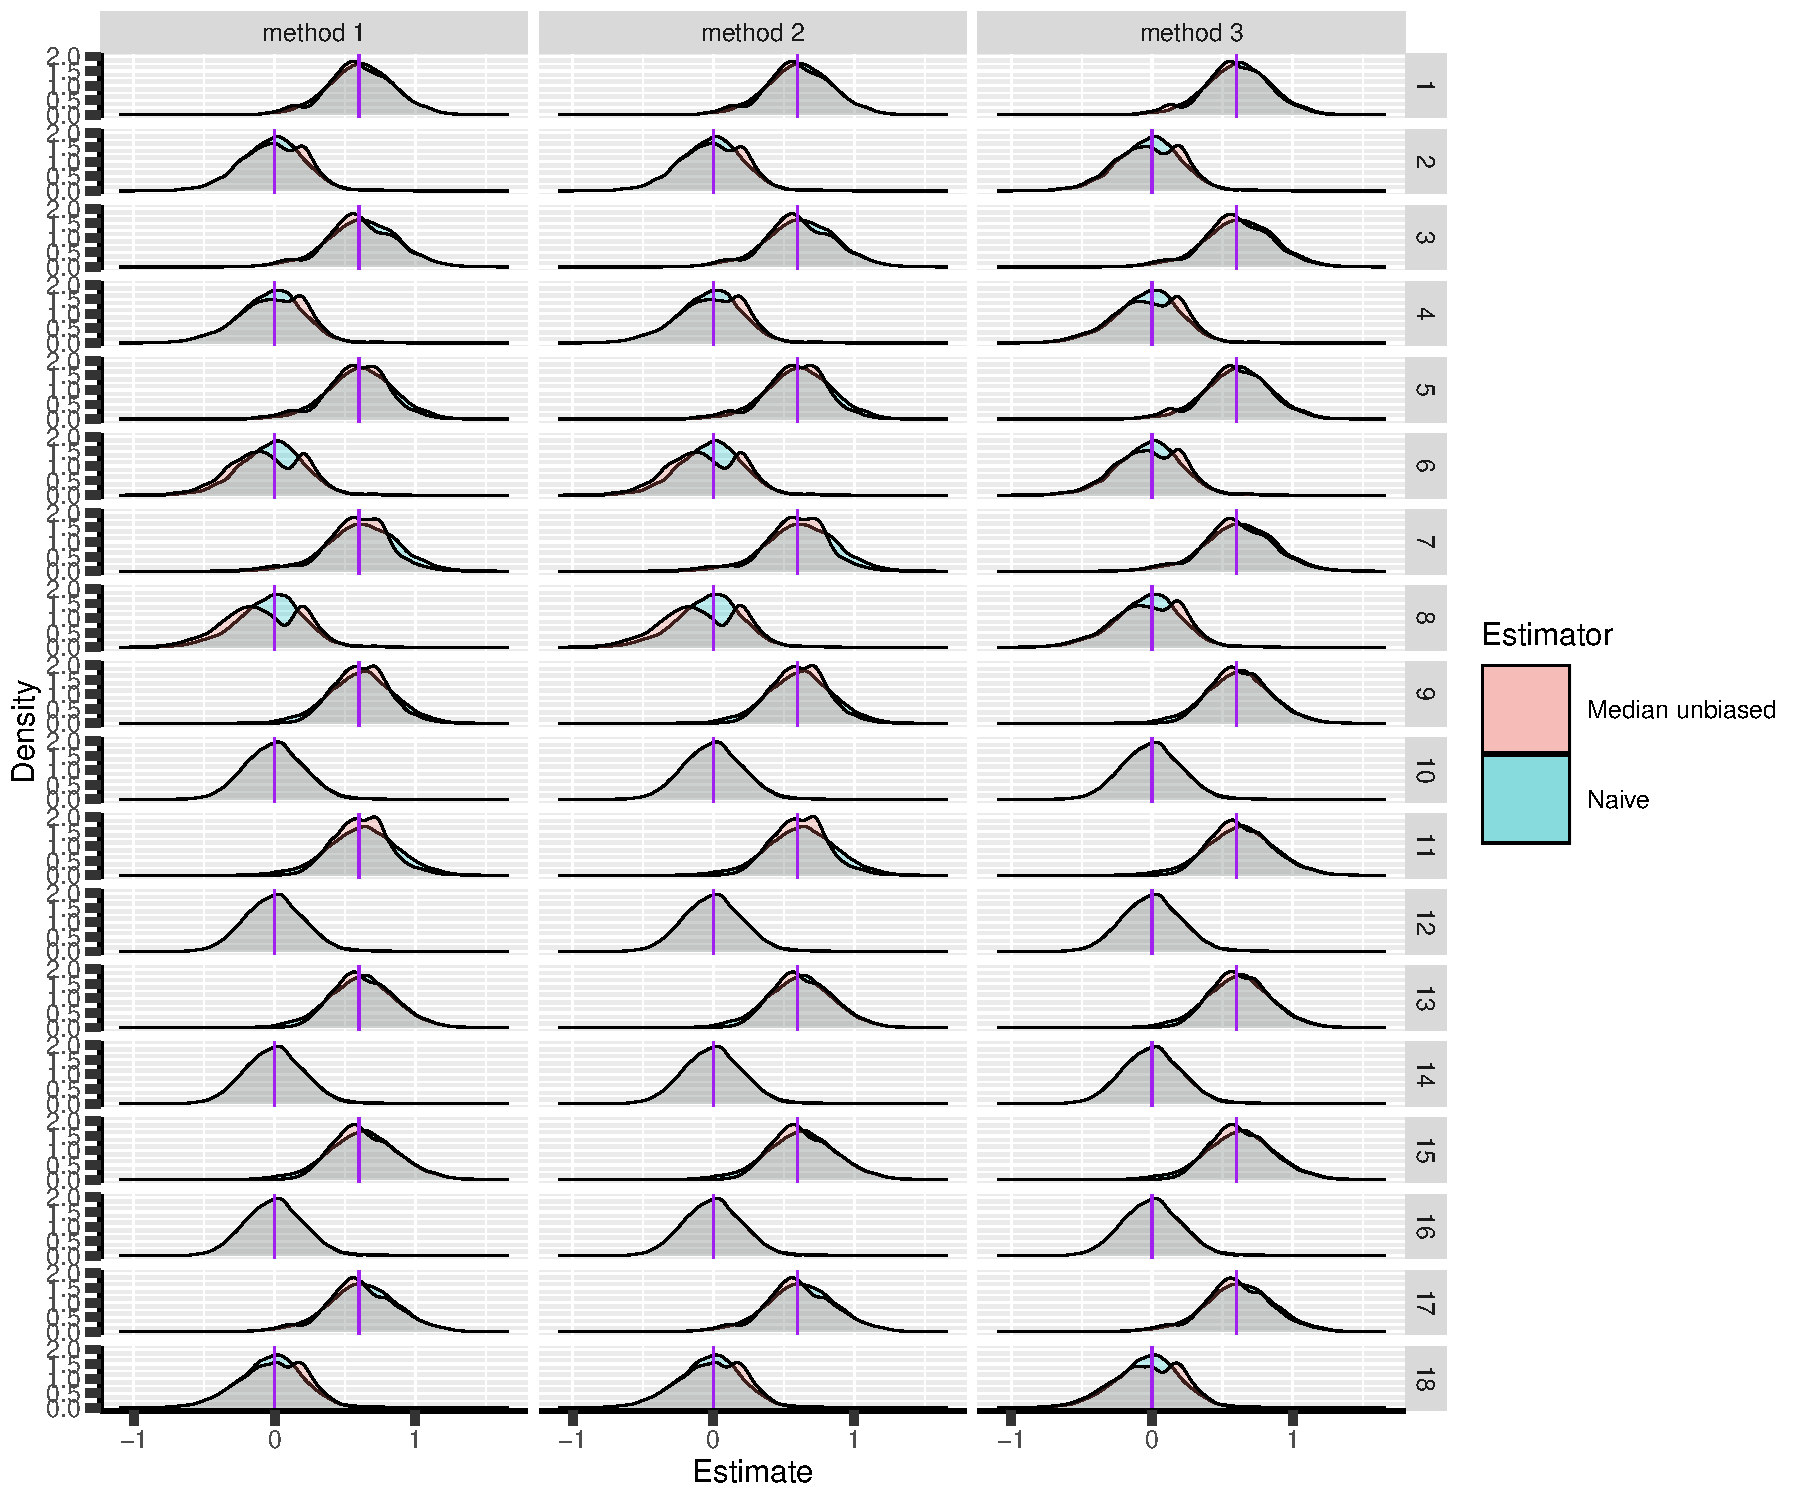
\includegraphics[trim={0 0 0 0},width=1\textwidth]{./figures/gg2stage-estimate-density.pdf}
\caption{Naive and Median unbiased estimate distribution over all simulations. Each row correspond to a different scenario}
\end{figure}

\begin{figure}[!h]
\centering
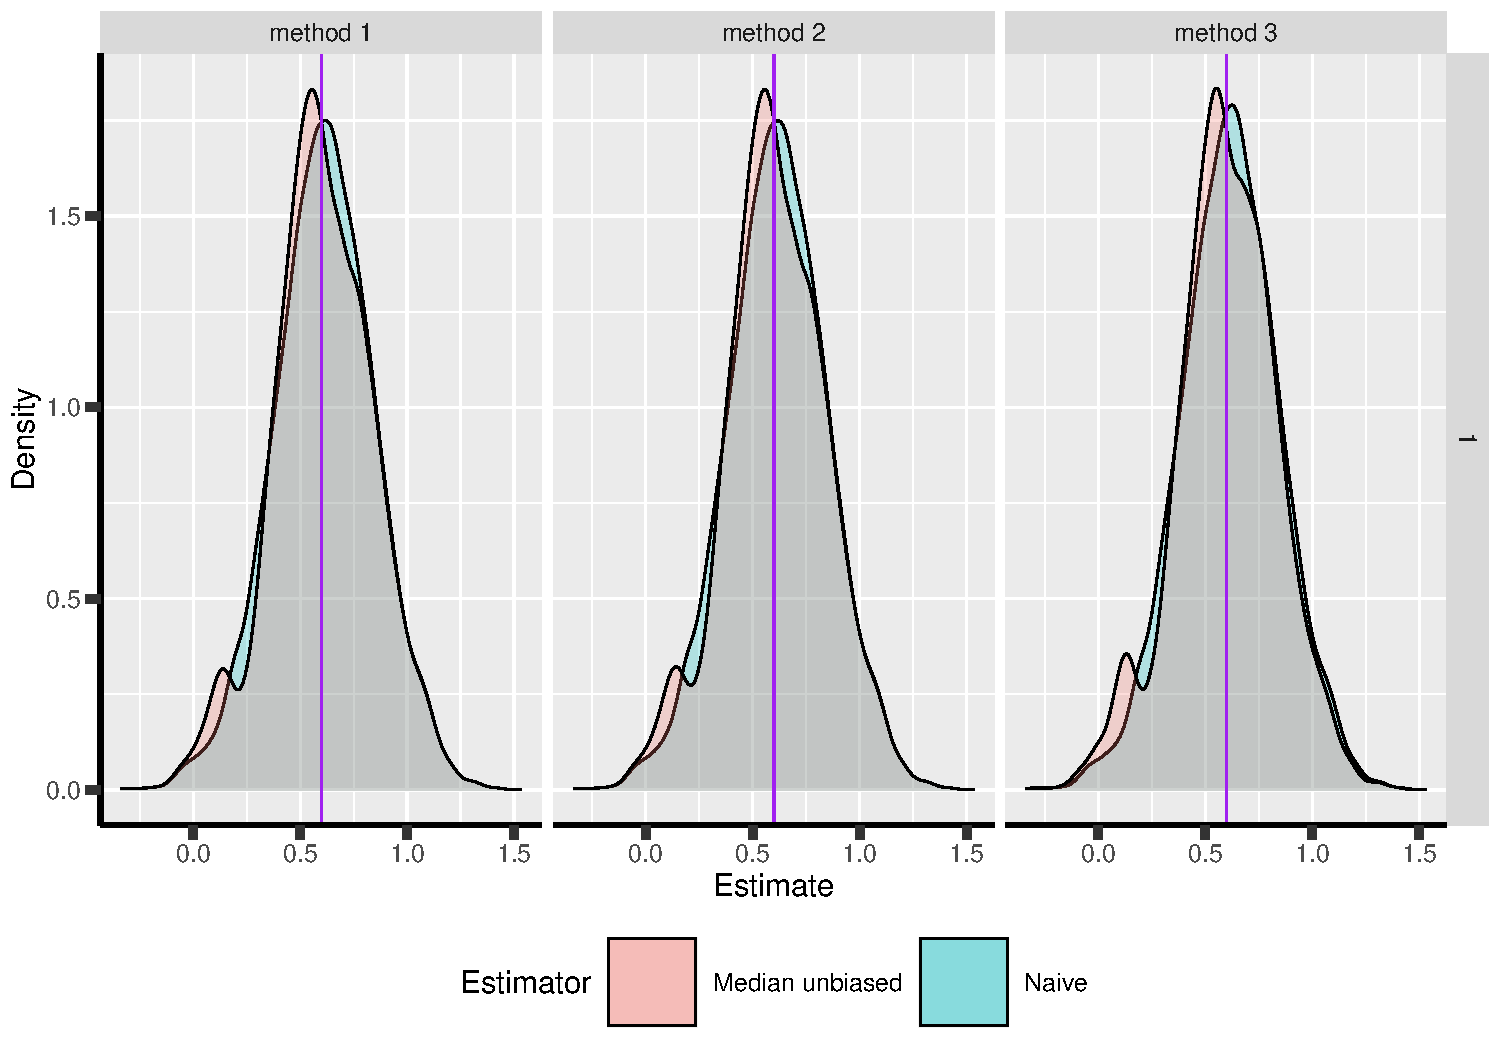
\includegraphics[trim={0 0 0 0},width=\textwidth]{./figures/gg2stage-estimate-density-scenario1.pdf}
\caption{Same but specific to scenario 1}
\end{figure}

\clearpage

Distribution of the median unbiased estimate conditional to the stage:
\begin{figure}[!h]
\centering
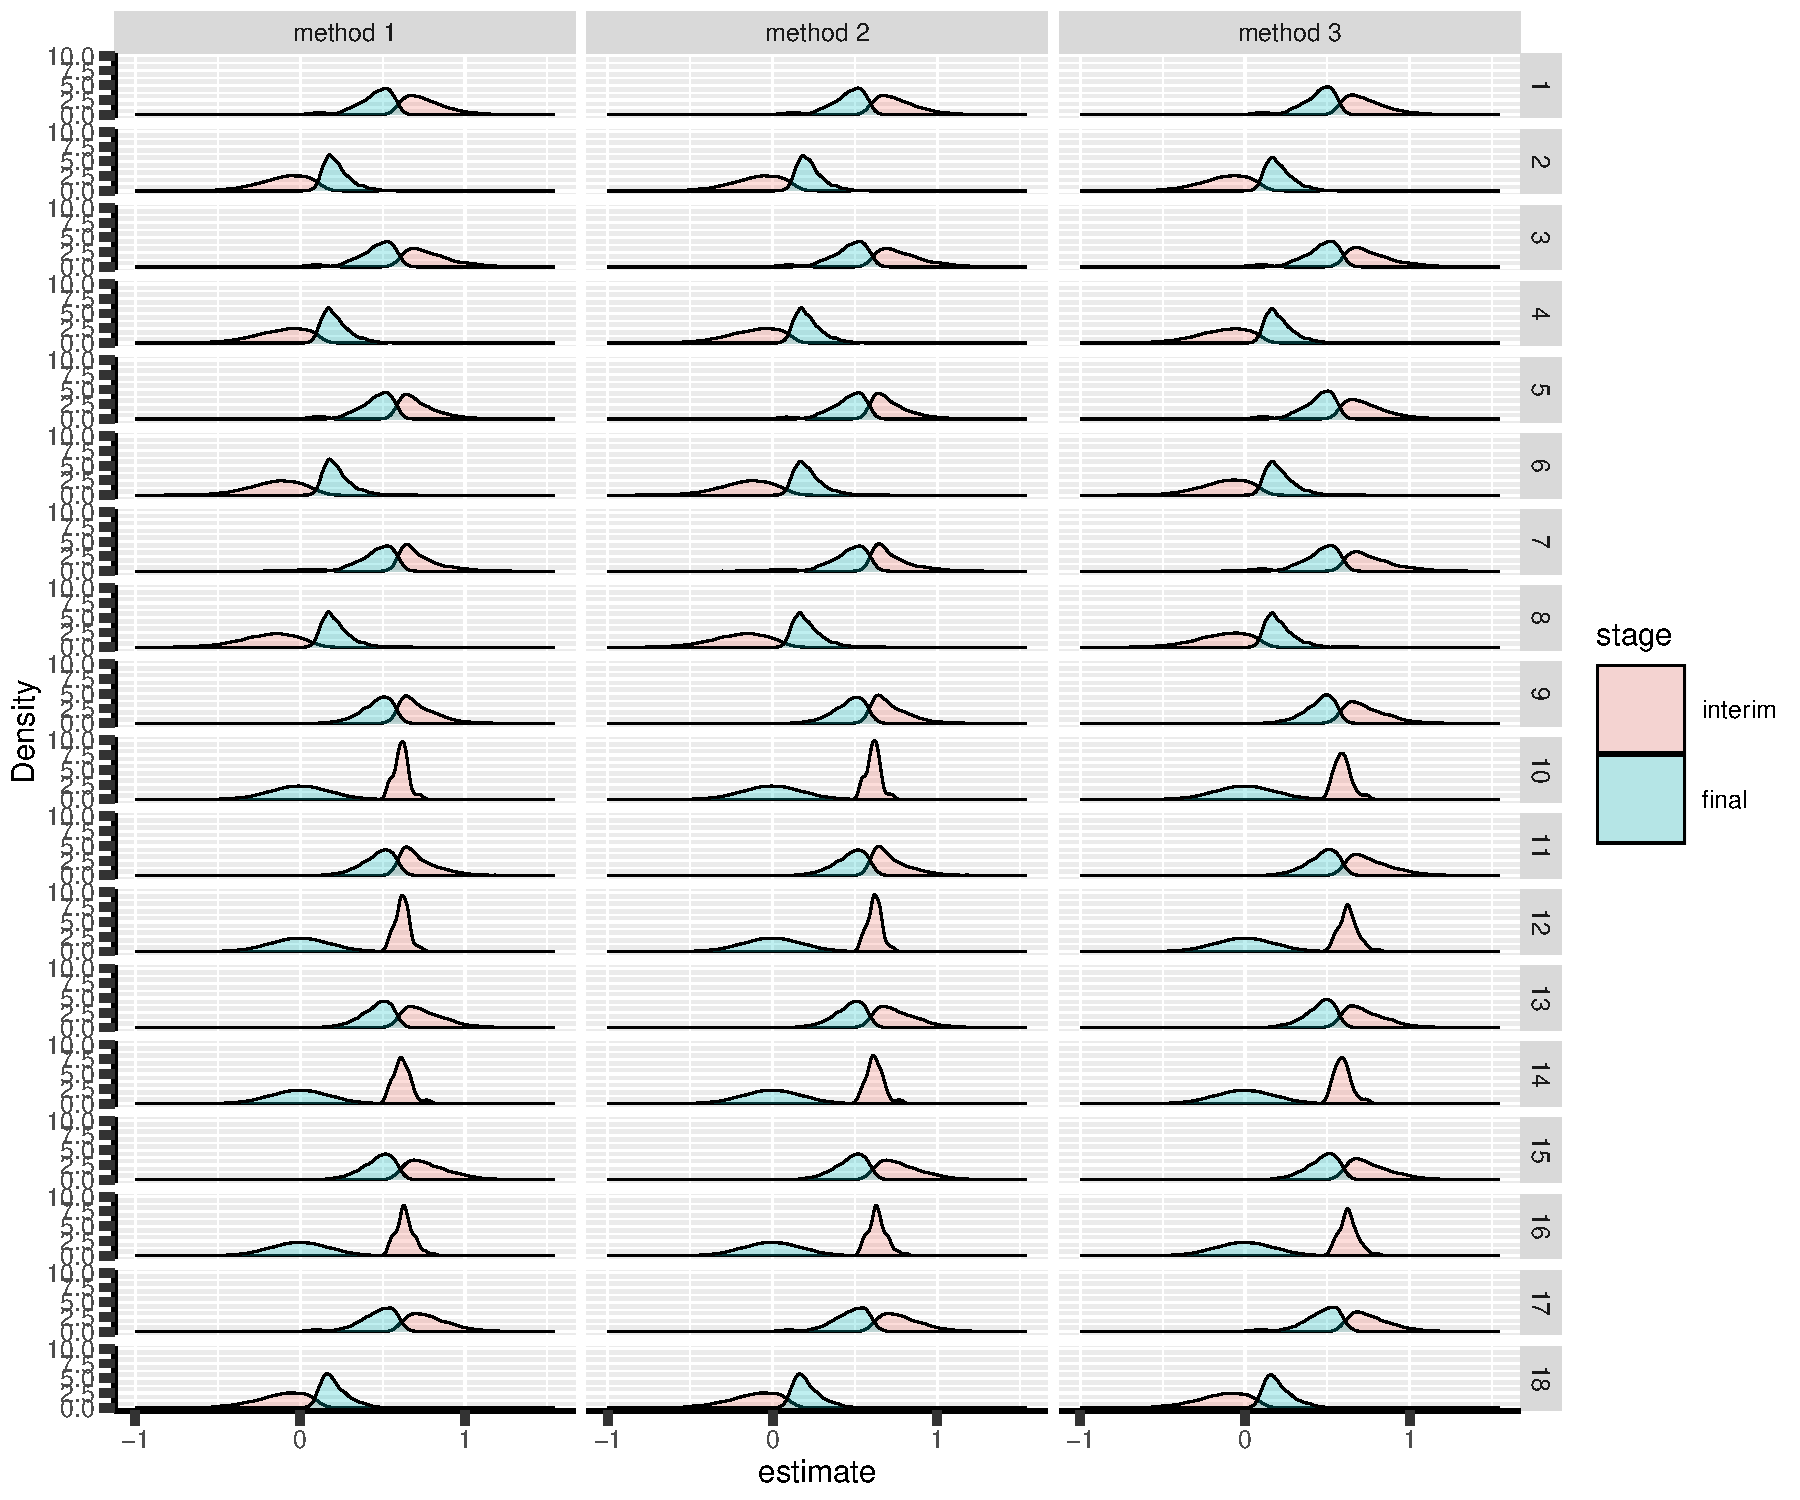
\includegraphics[trim={0 0 0 0},width=1\textwidth]{./figures/gg2stage-estimateC-density.pdf}
\caption{Median unbiased estimate distribution conditional to the stage. Each row correspond to a different scenario.}
\end{figure}

\clearpage

\subsection{3 stages}
\label{sec:org2393c92}

Distribution of the estimates:
\begin{figure}[!h]
\centering
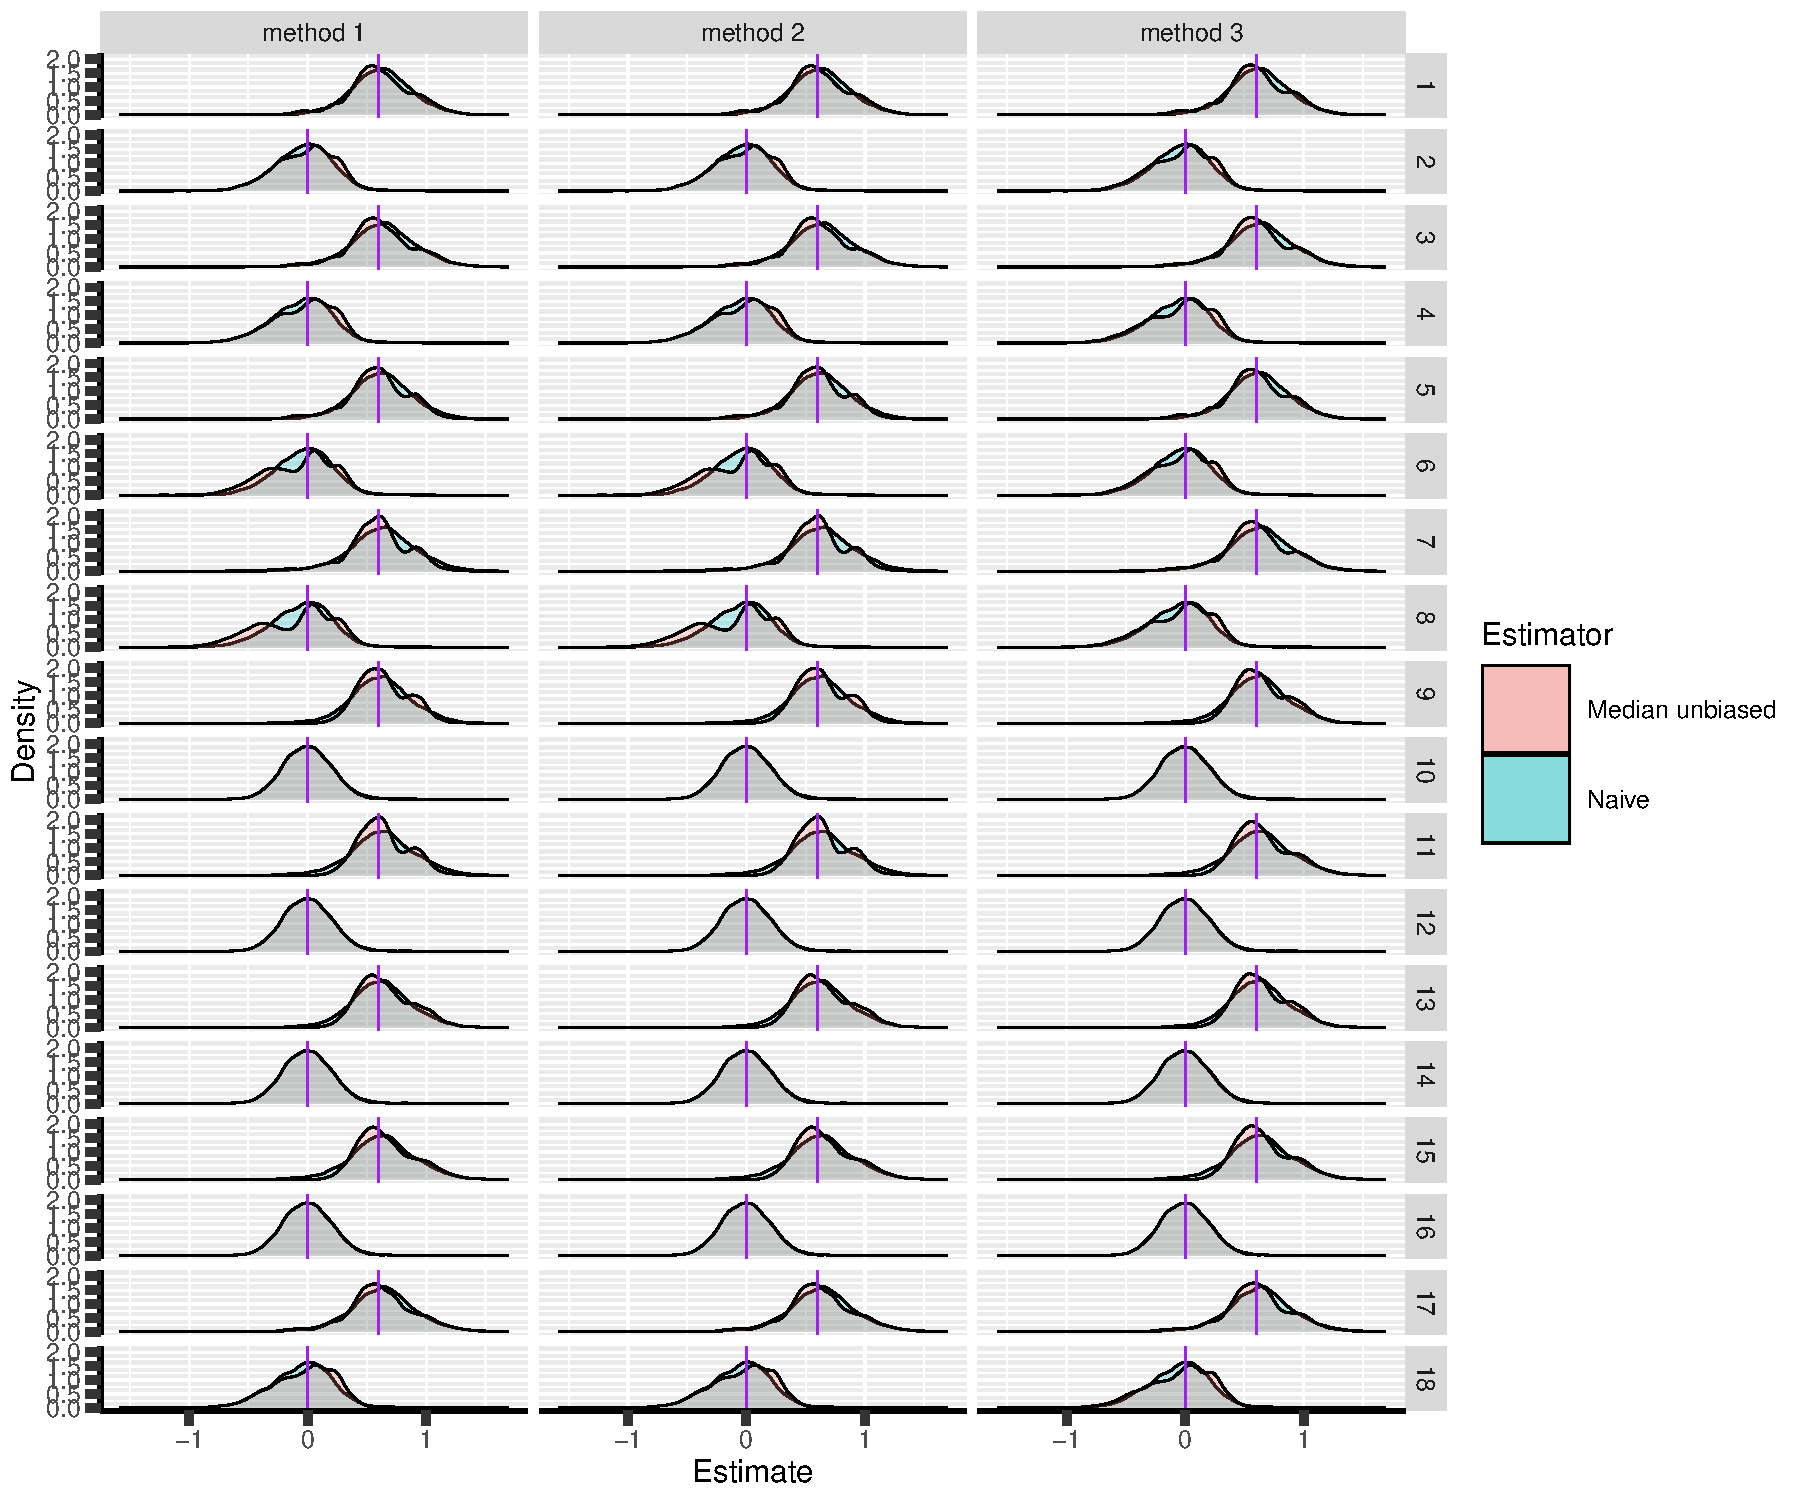
\includegraphics[trim={0 0 0 0},width=1\textwidth]{./figures/gg3stage-estimate-density.pdf}
\caption{Naive and Median unbiased estimate distribution over all simulations. Each row correspond to a different scenario}
\end{figure}

\begin{figure}[!h]
\centering
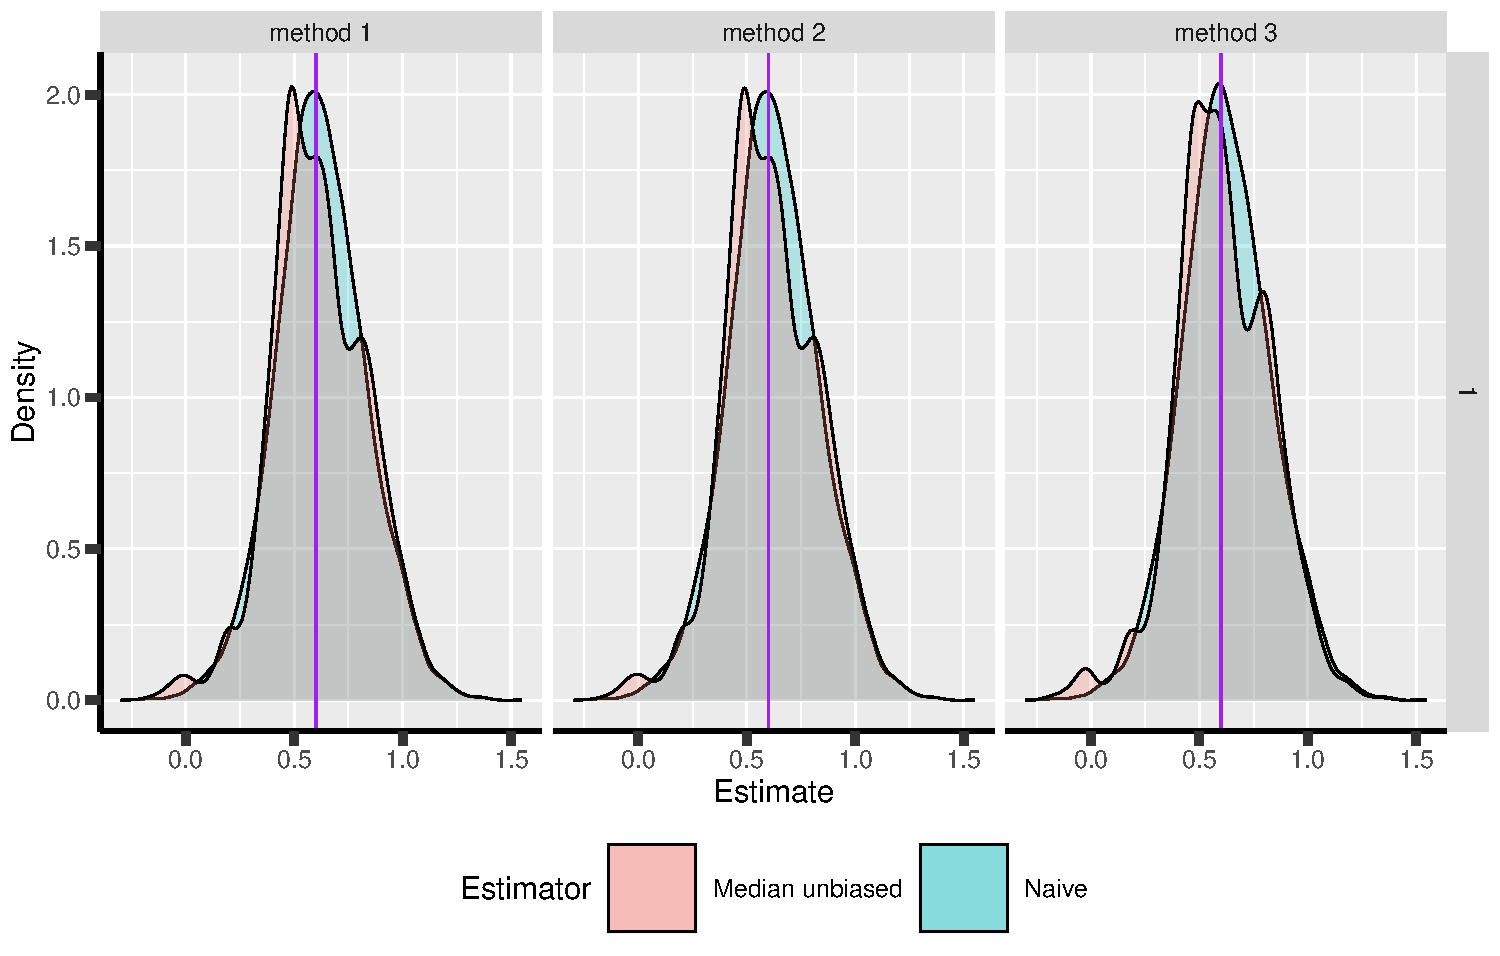
\includegraphics[trim={0 0 0 0},width=\textwidth]{./figures/gg3stage-estimate-density-scenario1.pdf}
\caption{Same but specific to scenario 1}
\end{figure}

\clearpage

Distribution of the median unbiased estimate conditional to the stage:
\begin{figure}[!h]
\centering
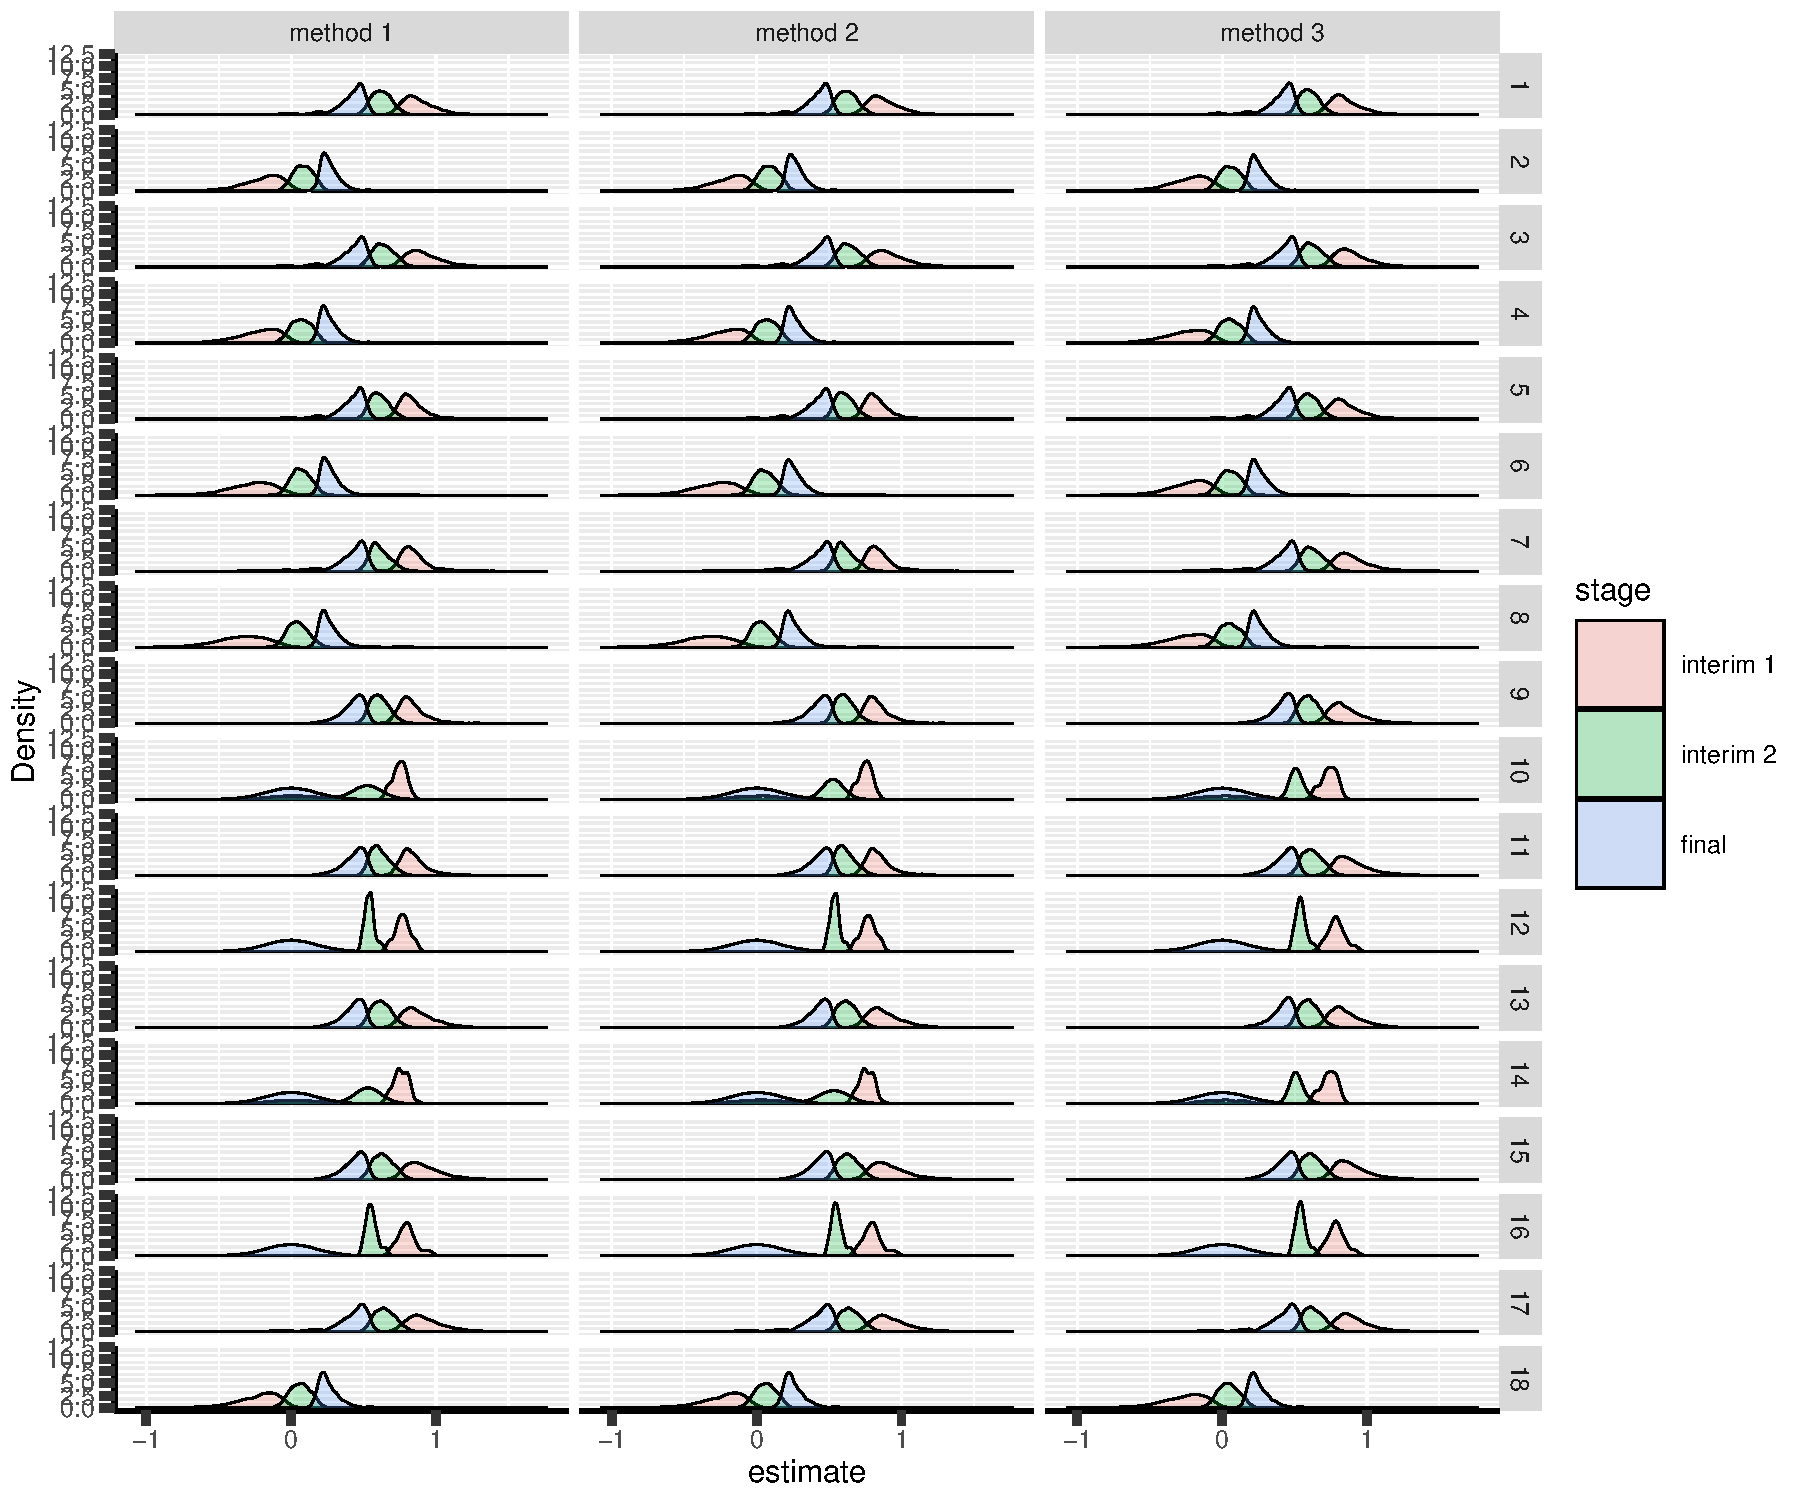
\includegraphics[trim={0 0 0 0},width=1\textwidth]{./figures/gg3stage-estimateC-density.pdf}
\caption{Median unbiased estimate distribution conditional to the stage. Each row correspond to a different scenario.}
\end{figure}

\clearpage

\section{Special cases}
\label{sec:orgc129d67}

\subsection{2 stages}
\label{sec:org4c0f4a6}

Reason for stopping (efficacy, futility, Imax reached), continuing the
trial (decreasing information, no boundary crossed), or concluding
(stop for futility at interim):
\begin{verbatim}
                                    scenario    1    2    3    4    5    6    7    8
reason                       method                                                 
efficacy                     1               5093   86 4874   80 5093   86 4874   80
                             2               5093   86 4874   81 5068   86 4861   77
                             3               5553  128 5028   91 5553  128 5028   91
futility                     1                320 7179  299 6950  320 7179  299 6950
                             2                349 7269  301 6960  274 6993  280 6803
                             3                242 6805  277 6776  242 6805  277 6776
no boundary crossed          1               4587 2735 4827 2970 4587 2735 4827 2970
                             2               4558 2645 4825 2959 4658 2921 4859 3120
                             3               4205 3067 4695 3133 4205 3067 4695 3133
stop for futility at interim 1                  0    0    0    0    0    0    0    0
                             2                  0    0    0    0    0    0    0    0
                             3                 10    3    0    0   10    3    0    0
\end{verbatim}

\begin{verbatim}
                                    scenario    9   10   11   12   13   14   15   16   17   18
reason                       method                                                           
efficacy                     1               5039   68 4821   64 5039   68 4821   64 4700   82
                             2               5028   67 4806   64 5039   68 4821   64 4700   82
                             3               5460   97 4959   72 5460   97 4959   72 4845   90
futility                     1                338 7164  309 6964  338 7164  309 6964  250 6719
                             2                301 6978  283 6833  359 7258  312 6973  250 6728
                             3                266 6800  279 6816  266 6800  279 6816  223 6532
no boundary crossed          1               4523 2768 4770 2972 4523 2768 4770 2972 5050 3099
                             2               4571 2955 4811 3103 4502 2674 4767 2963 5050 3090
                             3               4174 3103 4662 3112 4174 3103 4662 3112 4932 3278
stop for futility at interim 1                  0    0    0    0    0    0    0    0    0    0
                             2                  0    0    0    0    0    0    0    0    0    0
                             3                 15    0    0    0   15    0    0    0    1    0
\end{verbatim}

\clearpage

\subsection{3 stages}
\label{sec:org45e02c4}

Reason for stopping (efficacy, futility, Imax reached), continuing the
trial (decreasing information, no boundary crossed), or concluding
(stop for futility at interim):
\begin{verbatim}
                                    scenario     1     2     3     4     5     6     7     8
reason                       method                                                         
efficacy                     1                6306   115  6116   113  6306   115  6116   113
                             2                6305   115  6123   113  6275   114  6095   111
                             3                6785   155  6270   120  6785   155  6270   120
futility                     1                 444  8228   432  8078   444  8228   432  8078
                             2                 469  8306   434  8091   412  8102   393  7982
                             3                 357  7943   390  7966   357  7943   390  7966
Imax reached                 1                  14    10     0     0    14    10     0     0
                             2                  16    10     0     0     7     9     0     0
                             3                  10    11     0     0    10    11     0     0
no boundary crossed          1               10219  6864 10663  7277 10219  6864 10663  7277
                             2               10181  6743 10652  7260 10337  7246 10753  7513
                             3                9536  7480 10498  7521  9536  7480 10498  7521
stop for futility at interim 1                   0     0     0     0     0     0     0     0
                             2                   0     0     0     0     0     0     0     0
                             3                  24     2     3     0    24     2     3     0
\end{verbatim}

\begin{verbatim}
                                    scenario     9    10    11    12    13    14    15    16    17    18
reason                       method                                                                     
efficacy                     1                6334   116  6177   109  6334   116  6177   109  5961   101
                             2                6322   113  6160   107  6337   116  6182   110  5963   101
                             3                6782   156  6325   127  6782   156  6325   127  6105   110
futility                     1                 465 12836   438 12525   465 12836   438 12525   397  7896
                             2                 427 12493   398 12326   496 12946   442 12540   403  7911
                             3                 368 12227   395 12319   368 12227   395 12319   364  7768
Imax reached                 1                  14    22     0     0    14    22     0     0     0     0
                             2                  12    17     0     0    16    25     0     0     0     0
                             3                  12    22     0     0    12    22     0     0     0     0
no boundary crossed          1               10180  6839 10608  7323 10180  6839 10608  7323 10956  7684
                             2               10274  7192 10701  7526 10137  6726 10599  7307 10942  7666
                             3                9588  7400 10430  7507  9588  7400 10430  7507 10773  7957
stop for futility at interim 1                   0     0     0     0     0     0     0     0     0     0
                             2                   0     0     0     0     0     0     0     0     0     0
                             3                  27     0     1     0    27     0     1     0     0     0
\end{verbatim}

\clearpage

\section{Reversal probability}
\label{sec:orgeb5097b}

\subsection{2 stages}
\label{sec:orgfa886ed}


Percentage of time we observe a reversal:
\begin{verbatim}
        N  hypo missing ar binding  fixC fu2eff_1 fu2eff_2 fu2eff_3 eff2fu_1 eff2fu_2 eff2fu_3
 1: 10000 power    TRUE 10    TRUE FALSE    0.43%    0.50%        0    0.13%    0.14%    0.77%
 2: 10000 typeI    TRUE 10    TRUE FALSE    0.13%    0.13%        0    0.13%    0.13%    0.40%
 3: 10000 power    TRUE  5    TRUE FALSE    0.05%    0.05%        0    0.05%    0.05%    0.55%
 4: 10000 typeI    TRUE  5    TRUE FALSE    0.03%    0.03%        0    0.02%    0.02%    0.11%
 5: 10000 power    TRUE 10    TRUE  TRUE    0.24%    0.19%        0    0.37%    0.37%    0.77%
 6: 10000 typeI    TRUE 10    TRUE  TRUE    0.04%    0.04%        0    0.24%    0.24%    0.40%
 7: 10000 power    TRUE  5    TRUE  TRUE        0        0        0    0.40%    0.39%    0.55%
 8: 10000 typeI    TRUE  5    TRUE  TRUE        0        0        0    0.09%    0.08%    0.11%
 9:  9900 power    TRUE 10   FALSE  TRUE    0.21%    0.17%        0    0.49%    0.49%    0.76%
10: 10000 typeI    TRUE 10   FALSE  TRUE        0        0        0    0.23%    0.23%    0.36%
11:  9900 power    TRUE  5   FALSE  TRUE        0        0        0    0.35%    0.32%    0.47%
12: 10000 typeI    TRUE  5   FALSE  TRUE        0        0        0    0.09%    0.09%    0.13%
13:  9900 power    TRUE 10   FALSE FALSE    0.40%    0.46%        0    0.15%    0.16%    0.76%
14: 10000 typeI    TRUE 10   FALSE FALSE        0        0        0    0.08%    0.10%    0.36%
15:  9900 power    TRUE  5   FALSE FALSE    0.04%    0.05%        0    0.04%    0.04%    0.47%
16: 10000 typeI    TRUE  5   FALSE FALSE        0        0        0    0.02%    0.02%    0.13%
17: 10000 power   FALSE  5    TRUE FALSE    0.08%    0.08%        0    0.04%    0.04%    0.52%
18:  9900 typeI   FALSE  5    TRUE FALSE    0.02%    0.02%        0    0.03%    0.03%    0.14%
\end{verbatim}

\clearpage

\subsection{3 stages}
\label{sec:orgb9db3eb}

Percentage of time we observe a reversal:
\begin{verbatim}
        N  hypo missing ar binding  fixC fu2eff_1 fu2eff_2 fu2eff_3 eff2fu_1 eff2fu_2 eff2fu_3
 1: 10000 power    TRUE 10    TRUE FALSE    0.57%    0.66%        0    0.15%    0.19%    0.91%
 2: 10000 typeI    TRUE 10    TRUE FALSE    0.16%    0.18%        0    0.22%    0.22%    0.52%
 3: 10000 power    TRUE  5    TRUE FALSE    0.15%    0.16%        0    0.06%    0.06%    0.53%
 4: 10000 typeI    TRUE  5    TRUE FALSE    0.02%    0.02%        0    0.02%    0.02%    0.17%
 5: 10000 power    TRUE 10    TRUE  TRUE    0.37%    0.36%        0    0.61%    0.60%    0.91%
 6: 10000 typeI    TRUE 10    TRUE  TRUE    0.06%    0.04%        0    0.33%    0.32%    0.52%
 7: 10000 power    TRUE  5    TRUE  TRUE    0.05%    0.03%        0    0.37%    0.35%    0.53%
 8: 10000 typeI    TRUE  5    TRUE  TRUE    0.01%        0        0    0.12%    0.11%    0.17%
 9: 10000 power    TRUE 10   FALSE  TRUE    0.41%    0.39%        0    0.58%    0.56%    0.88%
10:  9931 typeI    TRUE 10   FALSE  TRUE        0        0        0    0.33%    0.30%    0.53%
11: 10000 power    TRUE  5   FALSE  TRUE    0.02%    0.01%        0    0.36%    0.35%    0.57%
12: 10000 typeI    TRUE  5   FALSE  TRUE        0        0        0    0.09%    0.08%    0.15%
13: 10000 power    TRUE 10   FALSE FALSE    0.66%    0.74%        0    0.24%    0.26%    0.88%
14:  9931 typeI    TRUE 10   FALSE FALSE        0        0        0    0.18%    0.21%    0.53%
15: 10000 power    TRUE  5   FALSE FALSE    0.10%    0.12%        0    0.07%    0.07%    0.57%
16: 10000 typeI    TRUE  5   FALSE FALSE        0        0        0    0.07%    0.07%    0.15%
17: 10000 power   FALSE  5    TRUE FALSE    0.11%    0.10%        0    0.07%    0.07%    0.53%
18: 10000 typeI   FALSE  5    TRUE FALSE    0.04%    0.04%        0    0.03%    0.03%    0.16%
\end{verbatim}


\clearpage

\section{Logical consistency of p-values/CIs}
\label{sec:orgaa659f9}

\subsection{Mismatch p-value / boundaries}
\label{sec:org063f6f5}
\subsubsection{2 stages}
\label{sec:orgc7b1f98}

When concluding for futility:
\begin{verbatim}
     hypo missing ar binding  fixC method 1 method 2 method 3
 1: power    TRUE 10    TRUE FALSE        0        0        0
 2: typeI    TRUE 10    TRUE FALSE        0        0        0
 3: power    TRUE  5    TRUE FALSE        0        0        0
 4: typeI    TRUE  5    TRUE FALSE        0        0        0
 5: power    TRUE 10    TRUE  TRUE        0        0        0
 6: typeI    TRUE 10    TRUE  TRUE        0        0        0
 7: power    TRUE  5    TRUE  TRUE        0        0        0
 8: typeI    TRUE  5    TRUE  TRUE        0        0        0
 9: power    TRUE 10   FALSE  TRUE        0        0        0
10: typeI    TRUE 10   FALSE  TRUE        0        0        0
11: power    TRUE  5   FALSE  TRUE        0        0        0
12: typeI    TRUE  5   FALSE  TRUE        0        0        0
13: power    TRUE 10   FALSE FALSE        0        0        0
14: typeI    TRUE 10   FALSE FALSE        0        0        0
15: power    TRUE  5   FALSE FALSE        0        0        0
16: typeI    TRUE  5   FALSE FALSE        0        0        0
17: power   FALSE  5    TRUE FALSE        0        0        0
18: typeI   FALSE  5    TRUE FALSE        0        0        0
\end{verbatim}

When concluding for efficacy:
\begin{verbatim}
     hypo missing ar binding  fixC method 1 method 2 method 3
 1: power    TRUE 10    TRUE FALSE        0        0        0
 2: typeI    TRUE 10    TRUE FALSE        0        0        0
 3: power    TRUE  5    TRUE FALSE        0        0        0
 4: typeI    TRUE  5    TRUE FALSE        0        0        0
 5: power    TRUE 10    TRUE  TRUE        0        0        0
 6: typeI    TRUE 10    TRUE  TRUE        0        0        0
 7: power    TRUE  5    TRUE  TRUE        0        0        0
 8: typeI    TRUE  5    TRUE  TRUE        0        0        0
 9: power    TRUE 10   FALSE  TRUE        0        0        0
10: typeI    TRUE 10   FALSE  TRUE        0        0        0
11: power    TRUE  5   FALSE  TRUE        0        0        0
12: typeI    TRUE  5   FALSE  TRUE        0        0        0
13: power    TRUE 10   FALSE FALSE        0        0        0
14: typeI    TRUE 10   FALSE FALSE        0        0        0
15: power    TRUE  5   FALSE FALSE        0        0        0
16: typeI    TRUE  5   FALSE FALSE        0        0        0
17: power   FALSE  5    TRUE FALSE        0        0        0
18: typeI   FALSE  5    TRUE FALSE        0        0        0
\end{verbatim}

\clearpage

\subsubsection{3 stages}
\label{sec:org716c857}

When concluding for futility:
\begin{verbatim}
     hypo missing ar binding  fixC method 1 method 2 method 3
 1: power    TRUE 10    TRUE FALSE        0        0        0
 2: typeI    TRUE 10    TRUE FALSE        0        0        0
 3: power    TRUE  5    TRUE FALSE        0        0    0.10%
 4: typeI    TRUE  5    TRUE FALSE        0    0.01%        0
 5: power    TRUE 10    TRUE  TRUE        0        0        0
 6: typeI    TRUE 10    TRUE  TRUE        0        0        0
 7: power    TRUE  5    TRUE  TRUE        0        0    0.10%
 8: typeI    TRUE  5    TRUE  TRUE        0        0        0
 9: power    TRUE 10   FALSE  TRUE        0        0        0
10: typeI    TRUE 10   FALSE  TRUE        0        0        0
11: power    TRUE  5   FALSE  TRUE    0.10%        0        0
12: typeI    TRUE  5   FALSE  TRUE        0        0        0
13: power    TRUE 10   FALSE FALSE        0        0        0
14: typeI    TRUE 10   FALSE FALSE        0        0        0
15: power    TRUE  5   FALSE FALSE    0.10%        0        0
16: typeI    TRUE  5   FALSE FALSE        0        0        0
17: power   FALSE  5    TRUE FALSE        0        0        0
18: typeI   FALSE  5    TRUE FALSE        0        0        0
\end{verbatim}

Largest mismatch:
\begin{verbatim}
[1] 0.02499104799
\end{verbatim}



When concluding for efficacy:
\begin{verbatim}
     hypo missing ar binding  fixC method 1 method 2 method 3
 1: power    TRUE 10    TRUE FALSE    0.01%        0        0
 2: typeI    TRUE 10    TRUE FALSE        0        0        0
 3: power    TRUE  5    TRUE FALSE        0        0        0
 4: typeI    TRUE  5    TRUE FALSE        0        0        0
 5: power    TRUE 10    TRUE  TRUE    0.01%        0        0
 6: typeI    TRUE 10    TRUE  TRUE        0        0        0
 7: power    TRUE  5    TRUE  TRUE        0        0        0
 8: typeI    TRUE  5    TRUE  TRUE        0        0        0
 9: power    TRUE 10   FALSE  TRUE        0        0        0
10: typeI    TRUE 10   FALSE  TRUE        0        0        0
11: power    TRUE  5   FALSE  TRUE        0        0        0
12: typeI    TRUE  5   FALSE  TRUE        0        0        0
13: power    TRUE 10   FALSE FALSE        0        0    0.01%
14: typeI    TRUE 10   FALSE FALSE        0        0        0
15: power    TRUE  5   FALSE FALSE        0        0        0
16: typeI    TRUE  5   FALSE FALSE        0        0        0
17: power   FALSE  5    TRUE FALSE        0        0        0
18: typeI   FALSE  5    TRUE FALSE        0        0        0
\end{verbatim}

Largest mismatch:
\begin{verbatim}
[1] 0.02500693409
\end{verbatim}


\clearpage

\subsection{Mismatch confidence intervals / boundaries}
\label{sec:orgfbfcda5}

\subsubsection{2 stages}
\label{sec:orgdb92a7a}

When concluding for futility:
\begin{verbatim}
     hypo missing ar binding  fixC       method 1       method 2       method 3
 1: power    TRUE 10    TRUE FALSE              0              0              0
 2: typeI    TRUE 10    TRUE FALSE              0              0              0
 3: power    TRUE  5    TRUE FALSE              0              0              0
 4: typeI    TRUE  5    TRUE FALSE              0              0              0
 5: power    TRUE 10    TRUE  TRUE              0              0              0
 6: typeI    TRUE 10    TRUE  TRUE              0              0              0
 7: power    TRUE  5    TRUE  TRUE              0              0              0
 8: typeI    TRUE  5    TRUE  TRUE              0              0              0
 9: power    TRUE 10   FALSE  TRUE 0 (NA: 37.73%) 0 (NA: 34.80%) 0 (NA: 35.93%)
10: typeI    TRUE 10   FALSE  TRUE  0 (NA: 0.24%)  0 (NA: 0.24%)  0 (NA: 0.37%)
11: power    TRUE  5   FALSE  TRUE 0 (NA: 35.87%) 0 (NA: 33.40%) 0 (NA: 34.53%)
12: typeI    TRUE  5   FALSE  TRUE  0 (NA: 0.09%)  0 (NA: 0.09%)  0 (NA: 0.13%)
13: power    TRUE 10   FALSE FALSE 0 (NA: 34.13%) 0 (NA: 35.61%) 0 (NA: 35.93%)
14: typeI    TRUE 10   FALSE FALSE  0 (NA: 0.08%)  0 (NA: 0.10%)  0 (NA: 0.37%)
15: power    TRUE  5   FALSE FALSE 0 (NA: 33.44%) 0 (NA: 33.62%) 0 (NA: 34.53%)
16: typeI    TRUE  5   FALSE FALSE  0 (NA: 0.02%)  0 (NA: 0.02%)  0 (NA: 0.13%)
17: power   FALSE  5    TRUE FALSE              0              0              0
18: typeI   FALSE  5    TRUE FALSE              0              0              0
\end{verbatim}

When concluding for efficacy:
\begin{verbatim}
     hypo missing ar binding  fixC method 1 method 2 method 3
 1: power    TRUE 10    TRUE FALSE        0        0        0
 2: typeI    TRUE 10    TRUE FALSE        0        0        0
 3: power    TRUE  5    TRUE FALSE        0        0        0
 4: typeI    TRUE  5    TRUE FALSE        0        0        0
 5: power    TRUE 10    TRUE  TRUE        0        0        0
 6: typeI    TRUE 10    TRUE  TRUE        0        0        0
 7: power    TRUE  5    TRUE  TRUE        0        0        0
 8: typeI    TRUE  5    TRUE  TRUE        0        0        0
 9: power    TRUE 10   FALSE  TRUE        0        0        0
10: typeI    TRUE 10   FALSE  TRUE        0        0        0
11: power    TRUE  5   FALSE  TRUE        0        0        0
12: typeI    TRUE  5   FALSE  TRUE        0        0        0
13: power    TRUE 10   FALSE FALSE        0        0        0
14: typeI    TRUE 10   FALSE FALSE        0        0        0
15: power    TRUE  5   FALSE FALSE        0        0        0
16: typeI    TRUE  5   FALSE FALSE        0        0        0
17: power   FALSE  5    TRUE FALSE        0        0        0
18: typeI   FALSE  5    TRUE FALSE        0        0        0
\end{verbatim}

\subsubsection{3 stages}
\label{sec:org5e4fe88}

When concluding for futility:
\begin{verbatim}
     hypo missing ar binding  fixC       method 1       method 2       method 3
 1: power    TRUE 10    TRUE FALSE              0              0              0
 2: typeI    TRUE 10    TRUE FALSE              0              0              0
 3: power    TRUE  5    TRUE FALSE              0              0              0
 4: typeI    TRUE  5    TRUE FALSE              0              0              0
 5: power    TRUE 10    TRUE  TRUE              0              0              0
 6: typeI    TRUE 10    TRUE  TRUE              0              0              0
 7: power    TRUE  5    TRUE  TRUE              0              0              0
 8: typeI    TRUE  5    TRUE  TRUE              0              0              0
 9: power    TRUE 10   FALSE  TRUE 0 (NA: 48.25%) 0 (NA: 45.63%) 0 (NA: 47.50%)
10: typeI    TRUE 10   FALSE  TRUE  0 (NA: 0.34%)  0 (NA: 0.31%)  0 (NA: 0.55%)
11: power    TRUE  5   FALSE  TRUE 0 (NA: 46.92%) 0 (NA: 43.72%) 0 (NA: 45.38%)
12: typeI    TRUE  5   FALSE  TRUE  0 (NA: 0.09%)  0 (NA: 0.08%)  0 (NA: 0.15%)
13: power    TRUE 10   FALSE FALSE 0 (NA: 45.00%) 0 (NA: 47.11%) 0 (NA: 47.50%)
14: typeI    TRUE 10   FALSE FALSE  0 (NA: 0.19%)  0 (NA: 0.22%)  0 (NA: 0.55%)
15: power    TRUE  5   FALSE FALSE 0 (NA: 44.89%) 0 (NA: 45.10%) 0 (NA: 45.38%)
16: typeI    TRUE  5   FALSE FALSE  0 (NA: 0.07%)  0 (NA: 0.07%)  0 (NA: 0.15%)
17: power   FALSE  5    TRUE FALSE              0              0              0
18: typeI   FALSE  5    TRUE FALSE              0              0              0
\end{verbatim}

When concluding for efficacy:
\begin{verbatim}
     hypo missing ar binding  fixC method 1 method 2 method 3
 1: power    TRUE 10    TRUE FALSE        0        0        0
 2: typeI    TRUE 10    TRUE FALSE        0        0        0
 3: power    TRUE  5    TRUE FALSE        0        0        0
 4: typeI    TRUE  5    TRUE FALSE        0        0        0
 5: power    TRUE 10    TRUE  TRUE        0        0        0
 6: typeI    TRUE 10    TRUE  TRUE        0        0        0
 7: power    TRUE  5    TRUE  TRUE        0        0        0
 8: typeI    TRUE  5    TRUE  TRUE        0        0        0
 9: power    TRUE 10   FALSE  TRUE        0        0        0
10: typeI    TRUE 10   FALSE  TRUE        0        0        0
11: power    TRUE  5   FALSE  TRUE        0        0        0
12: typeI    TRUE  5   FALSE  TRUE        0        0        0
13: power    TRUE 10   FALSE FALSE        0        0    0.01%
14: typeI    TRUE 10   FALSE FALSE        0        0        0
15: power    TRUE  5   FALSE FALSE        0        0        0
16: typeI    TRUE  5   FALSE FALSE        0        0        0
17: power   FALSE  5    TRUE FALSE        0        0        0
18: typeI   FALSE  5    TRUE FALSE        0        0        0
\end{verbatim}

\begin{verbatim}
[1] -1.665334537e-16
\end{verbatim}




\subsection{Range of p-values}
\label{sec:org9fa6c4b}

\subsubsection{2 stages}
\label{sec:org4f6d60c}
\begin{verbatim}
    missing binding  fixC ar  hypo   method 1   method 2   method 3
 1:    TRUE    TRUE FALSE 10 power [0;0.9163] [0;0.9163] [0;0.9163]
 2:    TRUE    TRUE FALSE 10 typeI      [0;1]      [0;1]      [0;1]
 3:    TRUE    TRUE FALSE  5 power [0;0.9194] [0;0.9194] [0;0.9202]
 4:    TRUE    TRUE FALSE  5 typeI      [0;1]      [0;1]      [0;1]
 5:    TRUE    TRUE  TRUE 10 power [0;0.9534] [0;0.9557] [0;0.9163]
 6:    TRUE    TRUE  TRUE 10 typeI      [0;1]      [0;1]      [0;1]
 7:    TRUE    TRUE  TRUE  5 power [0;0.9606] [0;0.9624] [0;0.9202]
 8:    TRUE    TRUE  TRUE  5 typeI  [1e-04;1]  [1e-04;1]      [0;1]
 9:    TRUE   FALSE  TRUE 10 power      [0;1]      [0;1]      [0;1]
10:    TRUE   FALSE  TRUE 10 typeI  [3e-04;1]  [4e-04;1]  [2e-04;1]
11:    TRUE   FALSE  TRUE  5 power      [0;1]      [0;1]      [0;1]
12:    TRUE   FALSE  TRUE  5 typeI  [3e-04;1]  [3e-04;1]  [1e-04;1]
13:    TRUE   FALSE FALSE 10 power      [0;1]      [0;1]      [0;1]
14:    TRUE   FALSE FALSE 10 typeI  [1e-04;1]  [1e-04;1]  [2e-04;1]
15:    TRUE   FALSE FALSE  5 power      [0;1]      [0;1]      [0;1]
16:    TRUE   FALSE FALSE  5 typeI  [1e-04;1]  [1e-04;1]  [1e-04;1]
17:   FALSE    TRUE FALSE  5 power  [0;0.867]  [0;0.867]  [0;0.882]
18:   FALSE    TRUE FALSE  5 typeI [0;0.9999] [0;0.9999]      [0;1]
\end{verbatim}

\clearpage

\subsubsection{3 stages}
\label{sec:orgd300419}
\begin{verbatim}
    missing binding  fixC ar  hypo       method 1       method 2   method 3
 1:    TRUE    TRUE FALSE 10 power     [0;0.8665]     [0;0.8663] [0;0.9035]
 2:    TRUE    TRUE FALSE 10 typeI [1e-04;0.9999] [1e-04;0.9999]  [2e-04;1]
 3:    TRUE    TRUE FALSE  5 power     [0;0.8959]     [0;0.8959] [0;0.9405]
 4:    TRUE    TRUE FALSE  5 typeI     [0;0.9998]     [0;0.9998] [0;0.9999]
 5:    TRUE    TRUE  TRUE 10 power      [0;0.935]     [0;0.9394] [0;0.9035]
 6:    TRUE    TRUE  TRUE 10 typeI      [3e-04;1]      [3e-04;1]  [2e-04;1]
 7:    TRUE    TRUE  TRUE  5 power      [0;0.965]     [0;0.9659] [0;0.9405]
 8:    TRUE    TRUE  TRUE  5 typeI          [0;1]      [1e-04;1] [0;0.9999]
 9:    TRUE   FALSE  TRUE 10 power          [0;1]          [0;1]      [0;1]
10:    TRUE   FALSE  TRUE 10 typeI      [4e-04;1]      [5e-04;1]  [3e-04;1]
11:    TRUE   FALSE  TRUE  5 power          [0;1]          [0;1]      [0;1]
12:    TRUE   FALSE  TRUE  5 typeI      [3e-04;1]      [4e-04;1]  [1e-04;1]
13:    TRUE   FALSE FALSE 10 power          [0;1]          [0;1]      [0;1]
14:    TRUE   FALSE FALSE 10 typeI      [1e-04;1]      [1e-04;1]  [3e-04;1]
15:    TRUE   FALSE FALSE  5 power          [0;1]          [0;1]      [0;1]
16:    TRUE   FALSE FALSE  5 typeI      [1e-04;1]      [1e-04;1]  [1e-04;1]
17:   FALSE    TRUE FALSE  5 power     [0;0.8745]     [0;0.8745]  [0;0.906]
18:   FALSE    TRUE FALSE  5 typeI     [0;0.9998]     [0;0.9998] [0;0.9999]
\end{verbatim}

\clearpage 

\section{Coverage}
\label{sec:orgcef8f64}
\subsection{2 stages}
\label{sec:org3b1cced}
\begin{verbatim}
     hypo missing ar binding  fixC           method 1           method 2           method 3
 1: power   FALSE  5    TRUE FALSE             95.32%             95.35%             95.50%
 2: power    TRUE  5   FALSE FALSE 96.06% (NA: 3.12%) 96.06% (NA: 3.14%) 96.26% (NA: 2.86%)
 3: power    TRUE  5   FALSE  TRUE 97.57% (NA: 3.47%) 97.56% (NA: 3.18%) 96.26% (NA: 2.86%)
 4: power    TRUE  5    TRUE FALSE             94.68%             94.69%             94.86%
 5: power    TRUE  5    TRUE  TRUE             95.98%             95.90%             94.86%
 6: power    TRUE 10   FALSE FALSE 96.16% (NA: 3.16%) 96.22% (NA: 3.32%) 95.96% (NA: 2.52%)
 7: power    TRUE 10   FALSE  TRUE 97.11% (NA: 3.70%) 97.07% (NA: 3.36%) 95.96% (NA: 2.52%)
 8: power    TRUE 10    TRUE FALSE             94.76%             94.75%             95.04%
 9: power    TRUE 10    TRUE  TRUE             95.55%             95.67%             95.04%
10: typeI   FALSE  5    TRUE FALSE             94.96%             94.96%             94.30%
11: typeI    TRUE  5   FALSE FALSE 95.02% (NA: 0.02%) 95.02% (NA: 0.02%) 95.11% (NA: 0.12%)
12: typeI    TRUE  5   FALSE  TRUE 95.09% (NA: 0.09%) 95.08% (NA: 0.09%) 95.11% (NA: 0.12%)
13: typeI    TRUE  5    TRUE FALSE             94.63%             94.63%             94.19%
14: typeI    TRUE  5    TRUE  TRUE             91.68%             91.52%             94.19%
15: typeI    TRUE 10   FALSE FALSE 95.09% (NA: 0.08%) 95.11% (NA: 0.10%) 95.29% (NA: 0.35%)
16: typeI    TRUE 10   FALSE  TRUE 95.23% (NA: 0.23%) 95.22% (NA: 0.23%) 95.29% (NA: 0.35%)
17: typeI    TRUE 10    TRUE FALSE             94.56%             94.57%             94.17%
18: typeI    TRUE 10    TRUE  TRUE             92.67%             92.39%             94.17%
\end{verbatim}

Average width of the confidence intervals
\begin{verbatim}
     hypo missing ar binding  fixC method 1 method 2 method 3
 1: power   FALSE  5    TRUE FALSE   1.0532   1.0533    1.053
 2: power    TRUE  5   FALSE FALSE   1.0453   1.0453    1.045
 3: power    TRUE  5   FALSE  TRUE   1.0520   1.0526    1.045
 4: power    TRUE  5    TRUE FALSE   1.0520   1.0520    1.051
 5: power    TRUE  5    TRUE  TRUE   1.0586   1.0587    1.051
 6: power    TRUE 10   FALSE FALSE   1.0559   1.0558    1.051
 7: power    TRUE 10   FALSE  TRUE   1.0638   1.0649    1.051
 8: power    TRUE 10    TRUE FALSE   1.0627   1.0631    1.058
 9: power    TRUE 10    TRUE  TRUE   1.0708   1.0712    1.058
10: typeI   FALSE  5    TRUE FALSE   1.0444   1.0443    1.047
11: typeI    TRUE  5   FALSE FALSE   0.9995   0.9995    1.014
12: typeI    TRUE  5   FALSE  TRUE   0.9994   0.9996    1.014
13: typeI    TRUE  5    TRUE FALSE   1.0431   1.0429    1.047
14: typeI    TRUE  5    TRUE  TRUE   1.0396   1.0406    1.047
15: typeI    TRUE 10   FALSE FALSE   1.0009   1.0009    1.044
16: typeI    TRUE 10   FALSE  TRUE   1.0005   1.0005    1.044
17: typeI    TRUE 10    TRUE FALSE   1.0469   1.0457    1.057
18: typeI    TRUE 10    TRUE  TRUE   1.0412   1.0425    1.057
\end{verbatim}

Average ratio between the length of the MUE CIs vs. the ML CIs
\begin{verbatim}
     hypo missing ar binding  fixC method 1 method 2 method 3
 1: power   FALSE  5    TRUE FALSE   1.0579   1.0580    1.058
 2: power    TRUE  5   FALSE FALSE   1.0539   1.0539    1.053
 3: power    TRUE  5   FALSE  TRUE   1.0602   1.0604    1.053
 4: power    TRUE  5    TRUE FALSE   1.0574   1.0574    1.057
 5: power    TRUE  5    TRUE  TRUE   1.0633   1.0632    1.057
 6: power    TRUE 10   FALSE FALSE   1.0603   1.0603    1.056
 7: power    TRUE 10   FALSE  TRUE   1.0680   1.0688    1.056
 8: power    TRUE 10    TRUE FALSE   1.0652   1.0656    1.060
 9: power    TRUE 10    TRUE  TRUE   1.0727   1.0730    1.060
10: typeI   FALSE  5    TRUE FALSE   1.0506   1.0506    1.054
11: typeI    TRUE  5   FALSE FALSE   0.9995   0.9995    1.014
12: typeI    TRUE  5   FALSE  TRUE   0.9996   0.9997    1.014
13: typeI    TRUE  5    TRUE FALSE   1.0499   1.0497    1.054
14: typeI    TRUE  5    TRUE  TRUE   1.0467   1.0477    1.054
15: typeI    TRUE 10   FALSE FALSE   1.0009   1.0010    1.045
16: typeI    TRUE 10   FALSE  TRUE   1.0008   1.0009    1.045
17: typeI    TRUE 10    TRUE FALSE   1.0502   1.0490    1.061
18: typeI    TRUE 10    TRUE  TRUE   1.0448   1.0461    1.061
\end{verbatim}

\clearpage

\subsection{3 stages}
\label{sec:org5c721db}

\begin{verbatim}
     hypo missing ar binding  fixC           method 1           method 2           method 3
 1: power   FALSE  5    TRUE FALSE             94.74% 94.73% (NA: 0.02%) 95.00% (NA: 0.01%)
 2: power    TRUE  5   FALSE FALSE 95.81% (NA: 4.35%) 95.85% (NA: 4.37%) 95.85% (NA: 3.85%)
 3: power    TRUE  5   FALSE  TRUE 97.75% (NA: 4.72%) 97.73% (NA: 4.32%) 95.86% (NA: 3.85%)
 4: power    TRUE  5    TRUE FALSE 95.11% (NA: 0.04%) 95.14% (NA: 0.04%) 95.32% (NA: 0.03%)
 5: power    TRUE  5    TRUE  TRUE 96.03% (NA: 0.03%) 96.15% (NA: 0.03%) 95.32% (NA: 0.03%)
 6: power    TRUE 10   FALSE FALSE 95.81% (NA: 4.23%) 95.89% (NA: 4.48%) 95.54% (NA: 3.21%)
 7: power    TRUE 10   FALSE  TRUE 97.48% (NA: 4.82%) 97.50% (NA: 4.44%) 95.52% (NA: 3.21%)
 8: power    TRUE 10    TRUE FALSE             95.15%             95.16%             95.33%
 9: power    TRUE 10    TRUE  TRUE             95.97%             95.91%             95.33%
10: typeI   FALSE  5    TRUE FALSE 94.80% (NA: 0.13%) 94.80% (NA: 0.13%) 94.19% (NA: 0.15%)
11: typeI    TRUE  5   FALSE FALSE 94.78% (NA: 0.30%) 94.83% (NA: 0.35%) 94.71% (NA: 0.40%)
12: typeI    TRUE  5   FALSE  TRUE 94.80% (NA: 0.32%) 94.79% (NA: 0.30%) 94.75% (NA: 0.40%)
13: typeI    TRUE  5    TRUE FALSE 95.05% (NA: 0.12%) 95.05% (NA: 0.12%) 94.20% (NA: 0.16%)
14: typeI    TRUE  5    TRUE  TRUE 89.80% (NA: 0.13%) 89.53% (NA: 0.15%) 94.20% (NA: 0.15%)
15: typeI    TRUE 10   FALSE FALSE 94.85% (NA: 0.42%) 94.90% (NA: 0.47%) 95.13% (NA: 0.77%)
16: typeI    TRUE 10   FALSE  TRUE 95.00% (NA: 0.57%) 95.01% (NA: 0.59%) 95.12% (NA: 0.79%)
17: typeI    TRUE 10    TRUE FALSE 95.02% (NA: 0.22%) 94.97% (NA: 0.14%) 94.30% (NA: 0.09%)
18: typeI    TRUE 10    TRUE  TRUE 91.52% (NA: 0.17%) 91.12% (NA: 0.14%) 94.30% (NA: 0.11%)
\end{verbatim}

Average width of the confidence intervals
\begin{verbatim}
     hypo missing ar binding  fixC method 1 method 2 method 3
 1: power   FALSE  5    TRUE FALSE   1.0789   1.0790    1.077
 2: power    TRUE  5   FALSE FALSE   1.0707   1.0707    1.069
 3: power    TRUE  5   FALSE  TRUE   1.0757   1.0757    1.069
 4: power    TRUE  5    TRUE FALSE   1.0782   1.0783    1.077
 5: power    TRUE  5    TRUE  TRUE   1.0834   1.0830    1.077
 6: power    TRUE 10   FALSE FALSE   1.1011   1.1012    1.096
 7: power    TRUE 10   FALSE  TRUE   1.1101   1.1110    1.096
 8: power    TRUE 10    TRUE FALSE   1.1085   1.1087    1.104
 9: power    TRUE 10    TRUE  TRUE   1.1176   1.1176    1.104
10: typeI   FALSE  5    TRUE FALSE   1.0788   1.0788    1.084
11: typeI    TRUE  5   FALSE FALSE   0.9997   0.9997    1.018
12: typeI    TRUE  5   FALSE  TRUE   0.9998   0.9998    1.018
13: typeI    TRUE  5    TRUE FALSE   1.0743   1.0742    1.079
14: typeI    TRUE  5    TRUE  TRUE   1.0755   1.0764    1.079
15: typeI    TRUE 10   FALSE FALSE   0.9995   0.9995    1.061
16: typeI    TRUE 10   FALSE  TRUE   0.9990   0.9994    1.061
17: typeI    TRUE 10    TRUE FALSE   1.1013   1.1005    1.114
18: typeI    TRUE 10    TRUE  TRUE   1.0942   1.0953    1.114
\end{verbatim}

Average ratio between the length of the MUE CIs vs. the ML CIs
\begin{verbatim}
     hypo missing ar binding  fixC method 1 method 2 method 3
 1: power   FALSE  5    TRUE FALSE   1.0825   1.0826    1.081
 2: power    TRUE  5   FALSE FALSE   1.0776   1.0776    1.076
 3: power    TRUE  5   FALSE  TRUE   1.0811   1.0808    1.076
 4: power    TRUE  5    TRUE FALSE   1.0827   1.0828    1.081
 5: power    TRUE  5    TRUE  TRUE   1.0859   1.0854    1.081
 6: power    TRUE 10   FALSE FALSE   1.1040   1.1041    1.098
 7: power    TRUE 10   FALSE  TRUE   1.1117   1.1120    1.098
 8: power    TRUE 10    TRUE FALSE   1.1100   1.1103    1.105
 9: power    TRUE 10    TRUE  TRUE   1.1173   1.1171    1.105
10: typeI   FALSE  5    TRUE FALSE   1.0854   1.0854    1.091
11: typeI    TRUE  5   FALSE FALSE   0.9996   0.9996    1.018
12: typeI    TRUE  5   FALSE  TRUE   0.9998   0.9997    1.018
13: typeI    TRUE  5    TRUE FALSE   1.0815   1.0814    1.087
14: typeI    TRUE  5    TRUE  TRUE   1.0844   1.0851    1.087
15: typeI    TRUE 10   FALSE FALSE   0.9995   0.9995    1.062
16: typeI    TRUE 10   FALSE  TRUE   0.9994   0.9996    1.062
17: typeI    TRUE 10    TRUE FALSE   1.1060   1.1052    1.120
18: typeI    TRUE 10    TRUE  TRUE   1.1006   1.1013    1.120
\end{verbatim}

\clearpage

\section{Percentage of missing values (2 stages)}
\label{sec:org47c16d4}

At the first interim
\begin{itemize}
\item \texttt{pc.all} percentage of observations with full data (with respect to
all observations, i.e. patients with baseline measurement)
\item \texttt{pc.missing3} percentage of observations missing the final outcome
but with intermediate outcome value and baseline.
\item \texttt{pc.missing23} percentage of observations with only baseline value
\end{itemize}

Here only for method 1 - values are very similar between different
methods:
\begin{verbatim}
    method missing ar  hypo  fixC binding     N pc.all pc.missing3 pc.missing23
 1:      1    TRUE  5 power FALSE    TRUE 10000  78.81       9.833       11.360
 2:      1    TRUE  5 typeI FALSE    TRUE 10000  78.81       9.833       11.360
 3:      1    TRUE  5 power  TRUE    TRUE 10000  78.81       9.833       11.360
 4:      1    TRUE  5 typeI  TRUE    TRUE 10000  78.81       9.833       11.360
 5:      1    TRUE  5 power  TRUE   FALSE  9900  78.73       9.861       11.410
 6:      1    TRUE  5 typeI  TRUE   FALSE 10000  78.73       9.860       11.410
 7:      1    TRUE  5 power FALSE   FALSE  9900  78.73       9.861       11.410
 8:      1    TRUE  5 typeI FALSE   FALSE 10000  78.73       9.860       11.410
 9:      1   FALSE  5 power FALSE    TRUE 10000  86.82       6.570        6.610
10:      1   FALSE  5 typeI FALSE    TRUE  9900  86.82       6.570        6.609
11:      1    TRUE 10 power FALSE    TRUE 10000  70.41      13.802       15.791
12:      1    TRUE 10 typeI FALSE    TRUE 10000  70.41      13.802       15.791
13:      1    TRUE 10 power  TRUE    TRUE 10000  70.41      13.802       15.791
14:      1    TRUE 10 typeI  TRUE    TRUE 10000  70.41      13.802       15.791
15:      1    TRUE 10 power  TRUE   FALSE  9900  70.42      13.807       15.776
16:      1    TRUE 10 typeI  TRUE   FALSE 10000  70.42      13.806       15.776
17:      1    TRUE 10 power FALSE   FALSE  9900  70.42      13.807       15.776
18:      1    TRUE 10 typeI FALSE   FALSE 10000  70.42      13.806       15.776
\end{verbatim}

\clearpage

\section{Information}
\label{sec:org3b3b288}

\subsection{2 stages}
\label{sec:org6c70a47}
Percentage of information for method 1\footnote{average over the reached stages}:
\begin{verbatim}
 scenario missing binding  fixC ar interim decision  final
        1    TRUE    TRUE FALSE 10   54.92    77.30 103.07
        2    TRUE    TRUE FALSE 10   54.92    77.05 102.89
        3    TRUE    TRUE FALSE  5   53.43    64.89 103.08
        4    TRUE    TRUE FALSE  5   53.43    64.61 102.94
        5    TRUE    TRUE  TRUE 10   54.92    77.30 103.07
        6    TRUE    TRUE  TRUE 10   54.92    77.05 102.89
        7    TRUE    TRUE  TRUE  5   53.43    64.89 103.08
        8    TRUE    TRUE  TRUE  5   53.43    64.61 102.94
        9    TRUE   FALSE  TRUE 10   54.72    76.74 102.63
       10    TRUE   FALSE  TRUE 10   54.71    76.11 103.18
       11    TRUE   FALSE  TRUE  5   53.25    64.47 102.68
       12    TRUE   FALSE  TRUE  5   53.25    64.35 103.18
       13    TRUE   FALSE FALSE 10   54.72    76.74 102.63
       14    TRUE   FALSE FALSE 10   54.71    76.11 103.18
       15    TRUE   FALSE FALSE  5   53.25    64.47 102.68
       16    TRUE   FALSE FALSE  5   53.25    64.35 103.18
       17   FALSE    TRUE FALSE  5   52.13    64.38 100.18
       18   FALSE    TRUE FALSE  5   52.12    64.19  99.81
\end{verbatim}

Similar results for other methods.

\subsection{3 stages}
\label{sec:org6b8d025}
Percentage of information for method 1\footnote{average over the reached stages}:
\begin{verbatim}
 scenario missing binding  fixC ar interim1 decision1 interim2 decision2 final3
        1    TRUE    TRUE FALSE 10    39.08     61.13    64.87     86.70 102.65
        2    TRUE    TRUE FALSE 10    39.08     61.04    64.66     86.27 102.16
        3    TRUE    TRUE FALSE  5    37.69     48.99    63.40     74.47 102.73
        4    TRUE    TRUE FALSE  5    37.69     48.93    63.17     74.09 102.19
        5    TRUE    TRUE  TRUE 10    39.08     61.13    64.87     86.70 102.65
        6    TRUE    TRUE  TRUE 10    39.08     61.04    64.66     86.27 102.16
        7    TRUE    TRUE  TRUE  5    37.69     48.99    63.40     74.47 102.73
        8    TRUE    TRUE  TRUE  5    37.69     48.93    63.17     74.09 102.19
        9    TRUE   FALSE  TRUE 10    38.85     60.43    64.52     85.88 102.34
       10    TRUE   FALSE  TRUE 10    38.85     61.18    64.76     90.06 102.97
       11    TRUE   FALSE  TRUE  5    37.47     48.55    63.08     73.93 102.43
       12    TRUE   FALSE  TRUE  5    37.47     49.96    63.30     75.12 103.00
       13    TRUE   FALSE FALSE 10    38.85     60.43    64.52     85.88 102.34
       14    TRUE   FALSE FALSE 10    38.85     61.18    64.76     90.06 102.97
       15    TRUE   FALSE FALSE  5    37.47     48.55    63.08     73.93 102.43
       16    TRUE   FALSE FALSE  5    37.47     49.96    63.30     75.12 103.00
       17   FALSE    TRUE FALSE  5    36.89     49.06    61.81     73.70  99.93
       18   FALSE    TRUE FALSE  5    36.89     48.91    61.69     73.42  99.67
\end{verbatim}
\end{document}